\documentclass[a4paper,12pt]{iitmdiss}

\usepackage{lscape}
\usepackage{graphicx}
\bibliographystyle{elsarticle-num}
\usepackage{tikz}
\usepackage[english]{babel}
\usepackage[autostyle]{csquotes}

\usetikzlibrary{positioning}
\usetikzlibrary{shapes,arrows}
\usepackage{listings}
\usepackage{geometry}
\usepackage{circuitikz}
\geometry{a4paper,left=25mm,top=20mm,right=25mm,bottom=20mm}
\colorlet{mygray}{black!30}
\colorlet{mygreen}{green!60!blue}
\colorlet{mymauve}{red!60!blue}

\usepackage[toc,page]{appendix}
\usepackage{steinmetz}
\usepackage{amsmath}



\lstset{
  backgroundcolor=\color{gray!10},  
  basicstyle=\small\ttfamily,
  columns=fullflexible,
  breakatwhitespace=false,      
  breaklines=true,                
  captionpos=b,                    
  commentstyle=\color{mygreen}, 
  extendedchars=true,              
  frame=single,                   
  keepspaces=true,             
  keywordstyle=\color{blue},      
  language=c++,                 
  numbers=none,                
  numbersep=3pt,                   
  numberstyle=\tiny\color{blue}, 
  rulecolor=\color{mygray},        
  showspaces=false,               
  showtabs=false,                 
  stepnumber=5,                  
  stringstyle=\color{mymauve},    
  tabsize=3,                      
  title=\lstname                
}




%%%%%%%%%%%%%%%%%%%%%%%%%%%%%%%%%%%%%%%%%%%%%%%%%%%%%%%%%%%%%%%%%%%%%%
% Title page

\title{Solar PV Inverter}
\degree{Bachelor of Technology}
\department{Electrical Engineering}
\submitted{June 2021}
\author{Yash Vardhan Omar, Satvik Patel}
\enrollment{171020012018, 171020011038}
\external{Dr. Manjunath K}
\addrexternal{Dept. of Electrical Engineering, IITRAM, Ahmedabad}
\internal{Dr. Kshitij Bhargava}
\addrinternal{Dept. of Electrical Engineering, IITRAM, Ahmedabad}
\adviser{Dr. Priyesh Chauhan}
\addradviser{Dept. of Electrical Engineering, IITRAM, Ahmedabad}
\coguide{Dr. ABC2}
\addrcoguide{Dept. of, IITRAM, Ahmedabad}
\chair{Name of the chairman}
\addrchair{Affiliation of the chairman}



%%%%%%%%%%%%%%%%%%%%%%%%%%%%%%%%%%%%%%%%%%%%%%%%%%%%%%%%%%%%%%%%%%%%%%
% Abstract

\abstract {Due to the increasing demand of renewable energy as a source of electricity, especially the solar energy, there arise a need to have a system that would work for both the on-grid and off-grid solar application , i.e., work as a hybrid system. The Project features a system that would control the flow of the power generated from PV module to the grid, household load and the battery system, depending on whether the grid is on-line or off-line, the battery needs charging or not. It has a MPPT and a PLL attached to it, which helps the system generate the maximum power possible and allows it to get connected with the grid. The SRF-PLL shown has been tested for a grid with variable frequency, phase and amplitude. It is also tested for a signal with harmonics that are usually found in the Indian transmission/distribution network. The efficiency of the MPPT and PLL approach is tested on off-line MATLAB Simulink and its implementation was tried on STM micro-controller.}

%%%%%%%%%%%%%%%%%%%%%%%%%%%%%%%%%%%%%%%%%%%%%%%%%%%%%%%%%%%%%%%%%%%%%%
% Acknowledgement
\acknowledgements{%Throughout this project we have received a great deal of support and guidance.

We would like to thank our supervisor, Dr. Priyesh Chauhan, who provided us the opportunity to work on this project. Your insightful feedback pushed us to sharpen our thinking and brought our work to a higher level. This Project helped us to gain more knowledge in the field of solar inverter and micro-controller. We would also like to thank Tejas Sir for helping us in this project.}

%%%%%%%%%%%%%%%%%%%%%%%%%%%%%%%%%%%%%%%%%%%%%%%%%%%%%%%%%%%%%%%%%%%%%%
% Dedication
\dedication{\begin{center}
    Dedicated to the almighty
\end{center}}

%%%%%%%%%%%%%%%%%%%%%%%%%%%%%%%%%%%%%%%%%%%%%%%%%%%%%%%%%%%%%%%%%%%%%%
% Nomenclature


\begin{document}
%%%%%%%%%%%%%%%%%%%%%%%%%%%%%%%%%%%%%%%%%%%%%%%%%%
% Introduction.

\chapter{Introduction}\label{chap:intro}
\pagenumbering{arabic}

The world's consumption of electrical energy is increasing at a rapid rate.
This increase has an impact on both developing and developed countries, as well as causing environmental issues. We live in a time when new power generation solutions are desperately needed; sources that are cleaner and more sustainable than traditional energy power plants that use oil, gas, and uranium. Renewable energy sources such as wind, geothermal, and photovoltaic energy are largely used in the solutions \textcolor{blue}{\cite{gammoudi2015stm}}. Electric power has been generated using energy from renewable natural resources such as solar, wind, rainfall, tidal, geothermal heat, and so on. Renewable energy (RE) sources have the following major advantages over conventional fossil energy sources (coal, oil, and natural gas): (1) they are refilled from natural resources; thus, they are sustainable and will never run out; (2) They emit very little or no carbon dioxide when they generate. To summarize, Renewable energy (RE) appears to be the most ideal and effective solution for dealing with environmental issues \textcolor{blue}{\cite{motahhir2018contribution}}.

Renewable Energy (RE) is seen as a critical and long-term solution to both transportation and power generating problems because the traditional energy is currently experiencing a depletion issue, and environmental contamination is on the rise. Rapid economic expansion necessitates the exploration, development of renewable energy sources. Solar energy has become a focused area as a type of new energy due to its in-exhaustible nature, safety, and cleanliness \textcolor{blue}{\cite{dengsheng2018research,cheddadi2018design}}. Photovoltaic energy or the solar energy is one of the renewable energy sources that is also environmentally friendly. Despite the large distance between the sun and the earth (150,106 km), the terrestrial layer receives a significant amount of energy from the sun (180,106 GW), which is sufficient to meet the world's energy need \textcolor{blue}{\cite{durgadevi2011study}}. Photovoltaic systems can be self-contained (water pumping, electric vehicles, public lighting, etc.) or grid-connected (power plants) \textcolor{blue}{\cite{gammoudi2015stm}}.

Photo voltaic (PV) system can be used used for obtaining the electricity by passing the DC supply from PV system through a inverter which would convert the incoming DC to AC which now can be utilised for fulfilling the electrical needs of world. Making maximum power point tracker (MPPT) is very much essential for this because the maximum power point (MPP) of a photo voltaic (PV) system fluctuates with changing climatic conditions (such as irradiance and temperature), so tracking the MPP accurately is an essential concern in the design of efficient PV systems \textcolor{blue}{\cite{tamkoriadesign}}.

In this Project work on solar pv inverter is done along with some controlling part like maximum power point tracker (MPPT), controller for switching on/off the supply between the pv module, grid, household load and the battery system, controller for phase locked loop (PLL). It has been tried to implement the same on the STM32F4 discovery board. Process of implementing the above mentioned ideas on STM32F4 discovery board is done using the waijung blockset and STM coding.

\section{Increasing demand of solar energy}
In recent years, the solar power business in India has emerged as a rapidly growing sector. It promotes the government's objective of long-term prosperity while also establishing itself as an important contributor to meeting the country's energy demands and a key role in ensuring energy security. Millions of people in Indian communities have profited from solar energy-based decentralized and distributed applications that satisfy their cooking, energy demands in a friendly manner. Reduced drudgery among rural women and girls involved in long-distance fuel wood collecting and cooking in smoky kitchens are among the social and economic benefits \textcolor{blue}{\cite{currentstatus|ministryofnewandrenewableenergy|governmentofindia}}.

Country’s solar potential of about 748 GW assuming 3 percent of the waste land area to be covered by Solar PV modules is assessed by the national institute of solar energy. National solar mission (NSM) is one of major mission in making solar energy take a central place in India's national plan towards climate change .This mission was launched on 11th January, 2010. Objective of this mission is to establish India as an international leader in solar energy by making effective policies for diffusion of solar technology across the country as quickly as possible. It targets of installing 100 GW solar plants which are grid connected by the year 2022. It is in line with INDC target to fulfil 40 \%  amassed electric power from renewable energy resources and to decrease the emission intensity  of its GDP by 33 to 35 percent from 2005 level by 2030 \textcolor{blue}{\cite{currentstatus|ministryofnewandrenewableenergy|governmentofindia}}.

\section{Brief on Off and On Grid  Solar PV programme}
\subsection{Off-grid Solar PV Programme}
It is one of the oldest programme of ministry aimed to provide solar energy in areas where grid power is not proper or on which one cannot depend fully. A target of acheiving 2000 MWp for off-grid solar pv applications was kept under the NSM scheme. Off-grid applications includes solar home lighting systems, solar pumps, solar study lamps, solar power plants etc \textcolor{blue}{\cite{mnre}}. The number of units of off-grid solar pv applications installed up till 2018-19 is shown in Table \ref{tab:1.1}. 

 \begin{table}[hbt!]
    \centering
    \caption{Number of units of off-grid solar pv applications.}
    \label{tab:my_label}
    \begin{tabular}{|c|c|}
    \hline
    \textbf{System}  &\textbf{No. of units/capacity installed}  \\ \hline
    Solar Lantern/ Lamp & 5823800 \\ \hline
    			
    Solar Home lighting & 1715214 \\  \hline
    Solar street light & 659218 \\  \hline
    Solar Pump & 237120  \\  \hline
    Solar stand alone (KWp) & 212054.2 \\ \hline
\end{tabular}
\label{tab:1.1}
\end{table}



\subsection{On-grid Solar PV Programme}
100 GW  of grid connected solar power has been put as a target to acheive it by 2022. Goverment of India (GOI) has formulated many policies and launched many schemes to encourage the generation of solar power in India so that it acheives the target by 2022. Some of the schemes are solar park scheme, CPSU scheme, canal top scheme and many more. India has achieved 5th rank for solar power development in the world \textcolor{blue}{\cite{mnre1}}. The cumulative capacity of on-grid solar power from year 2015-19 is shown in Table \ref{tab:1.2}.

\begin{table}[hbt!]
    \centering
    \caption{Cumulative capacity of on-grid solar power.}
    \begin{tabular}{|c|c|c|c|}
    \hline
     Sr. No. &\textbf{Year} &\textbf{Capacity added during F.Y (MW)} &\textbf{Cumulative capacity (MW)}  \\ \hline
     1 & 2015-16 & 3018.88 & 6762.87 \\ \hline
     2 & 2016-17 & 5525.98 & 12288.85 \\ \hline
     3 & 2017-18 & 9362.63 & 21651.48 \\ \hline
     4 & 2018-19 & 6529.20 & 28180.68 \\ \hline
    \end{tabular}
    \label{tab:1.2}
    \end{table}

\chapter{Solar Energy}\label{chap:solar energy}
\section{What is Solar energy ?}
Solar energy is the heat from the Sun that can be captured using a variety of technologies including solar heating, solar thermal energy, photovoltaics, solar architecture, artificial photosynthesis and molten salt power plants. It is an important source of renewable energy, and depending on how it captures and distributes solar energy or converts it to solar power, its technologies are classified as passive or active solar.

To harness the energy, active solar solutions include photovoltaic systems, solar water heating and concentrated solar power. Orienting a structure to the Sun, selecting materials with light dispersing qualities or favorable thermal mass and creating rooms that naturally circulate air are all examples of passive solar approaches \textcolor{blue}{\cite{wikipedia_2021}}. 

\section{Working of Solar cell.}
Alexandre-Edmond Becquerel was the first one to observe the photo-voltaic effect in 1839 \textcolor{blue}{\cite{castellano2010solar}}. The first modern solar cell was made in 1946 by Russel Ohl and was made of silicon \textcolor{blue}{\cite{castellano2010solar,yadav2015enhancement}}. The photo-voltaic technology is based on principle of electron-hole pair creation in the cell. The cell is composed of two layers consisting of p-type and n-type material as shown in Figure \ref{fig:2.1}.

The layer with excess of electrons and deficiency of holes is the n layer and the layer with excess of holes and deficiency of electrons is the p layer. Whenever the sun rays fall on the surface of solar cell, a current starts flowing from the p layer to the n layer due to movement of electrons and holes, thus powering the load. Between the p and n layer a depletion region also called P-N junction is formed due to combination of minority charge carriers (electrons in case of p layer and holes in case of n layer). The width of depletion region affects the current flow because a strong electric field will develop in the depletion region due to more combination of holes and electron which will oppose current flow. 

\begin{figure}[hbt!]
    \centering
    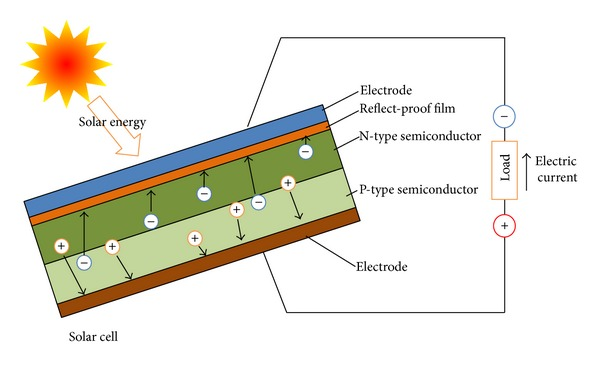
\includegraphics[height=8cm,width=15cm]{Schematic-operating-principle-of-a-PV-solar-cell-adapted-from-22.jpg}
    \caption{Schematic representation of Solar Cell (adapted from \textcolor{blue}{\cite{zhang2014photovoltaics,stevenson53slimmer}})}
    \label{fig:2.1}
\end{figure}


\section{Electrical Modelling of solar cell.}
Solar cell can be represented in the form of a electric circuit as shown in the Figure \ref{fig:2.2}. The solar cells are semiconductor devices that resembles the characteristics of a diode. The value of $I_o$ and $V_o$ is approximately 1 to 3 amps and 0.5 volt respectively.

The output current and voltage of the solar cell gets affected due to the change in irradiance (intensity of light rays falling) and temperature. The I-V characterstics of the cell at various values of irradiance and temperature is shown in the Figure \ref{fig:2.3}, \ref{fig:2.4} respectively. In Figure \ref{fig:2.3} current (I) has a considerable change as the value of irradiance (G) changes whereas in Figure \ref{fig:2.4} voltage has a considerable change due to change in temperature. As the irradiance decreases the current output from the solar cell also decreases and as the temperature decreases, output voltage of the solar cell increases. So in order to obtain maximum power from the solar cell, the operation of solar cell needs to be done at maximum power point (MPP) shown in Figure \ref{fig:2.3} and \ref{fig:2.4}.

\begin{figure}[hbt!]
\centering
\begin{circuitikz}
\draw
(0,0) to[american current source] (0,4) -- (2,4) to[full diode] (2,0) -- (0,0)

(2,4) -- (4,4) to[american resistor,l=$R_p$] (4,0) -- (2,0) -- (0,0)

(4,4) to[american resistor,l_=$R_s$,i_=$I_o$] (8,4) to[voltmeter,l=$V_o$] (8,0) -- (0,0);

\end{circuitikz}
\caption{Simplified Circuit Model of a Solar Cell}
\label{fig:2.2}
\end{figure}

\begin{figure}[hbt!]
    \centering
    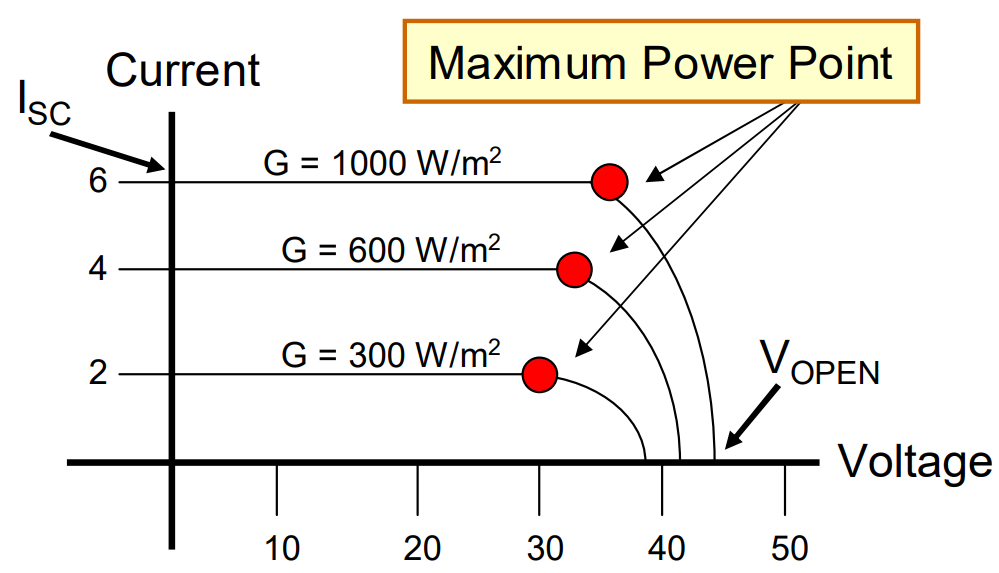
\includegraphics[width=10.8cm,height=8cm]{IV1.png}
    \caption{I-V characterstics for different value of irradiation (adapted from \textcolor{blue}{\cite{kamil2010grid}})}
    \label{fig:2.3}
\end{figure}

\begin{figure}[hbt!]
    \centering
    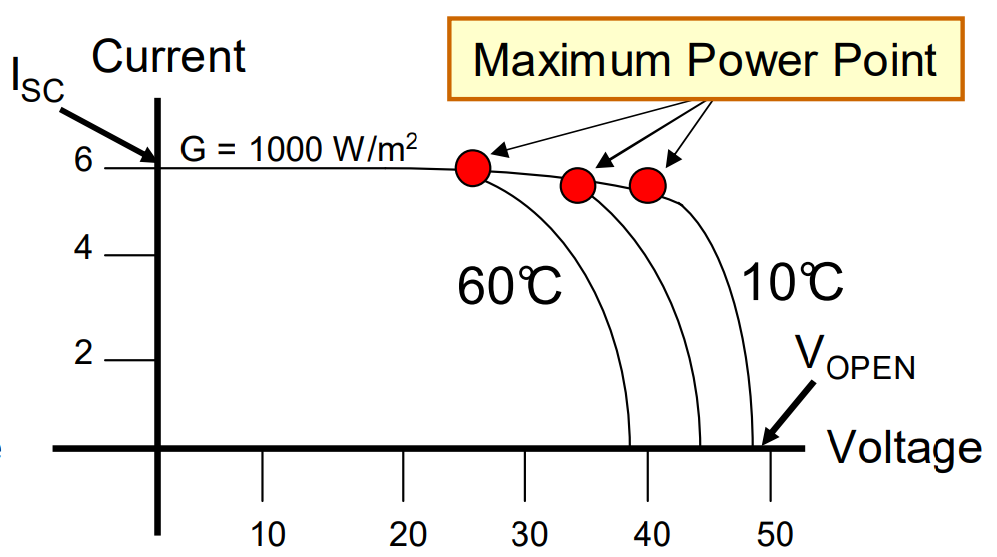
\includegraphics[width=10.8cm,height=8cm]{IV2.png}
    \caption{I-V characaterstics for different value of temperature (adapted from \textcolor{blue}{\cite{kamil2010grid}})}
    \label{fig:2.4}
\end{figure}

\section{MATLAB Simulink model of Solar cell}
The simulink model of solar cell is developed and shown in Figure \ref{fig:2.5}. The I-V characterstics of the solar cell made in simulink is shown in Figure \ref{fig:2.6} and \ref{fig:2.7}. Thus results of Figure \ref{fig:2.3}, \ref{fig:2.4} were practically verified .

\begin{figure}[hbt!]
    \centering
    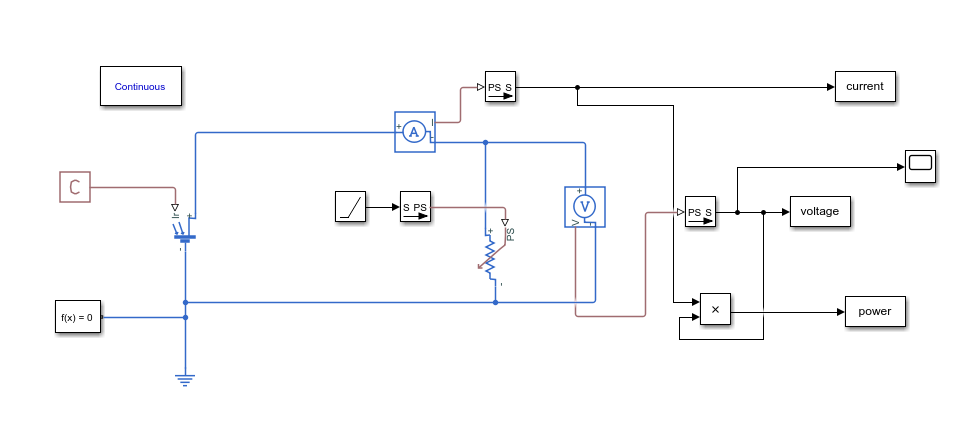
\includegraphics[width=17cm,height=9cm]{Solar Pv simulink(1).png}
    \caption{Simulink model of a solar cell}
    \label{fig:2.5}
\end{figure}

\begin{figure}[hbt!]
    \centering
    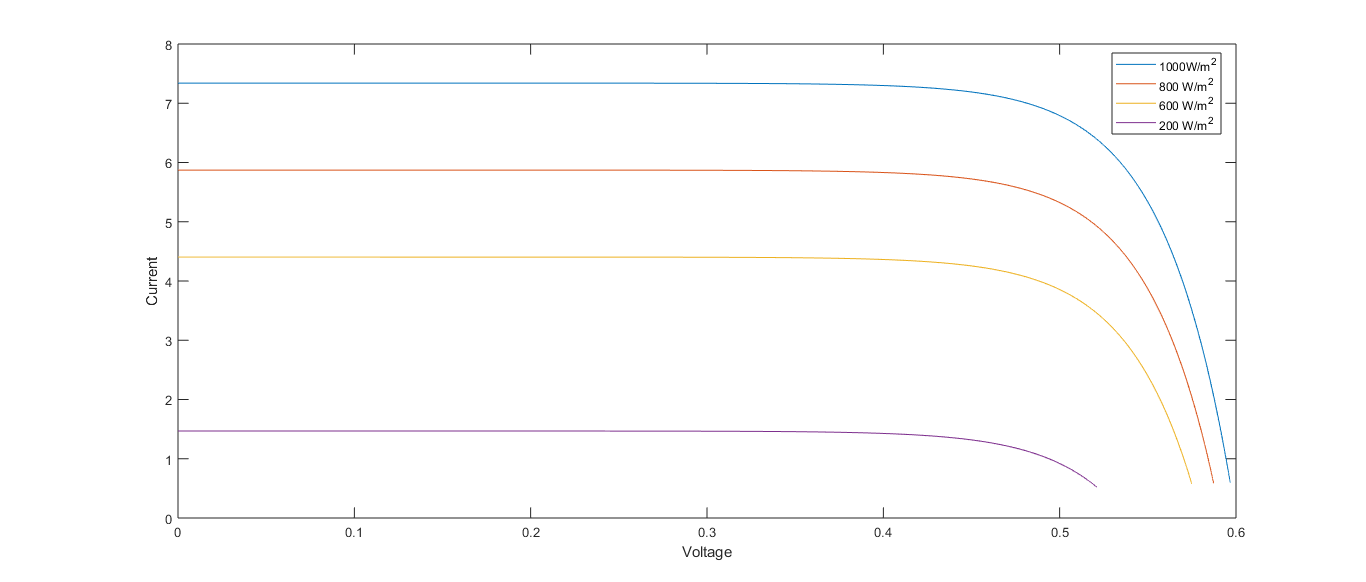
\includegraphics[width=16cm,height=9cm]{I-V for diff intensity(1).png}
    \caption{I-V characterstics for different value of Intensity}
    \label{fig:2.6}
\end{figure}

\begin{figure}[hbt!]
    \centering
    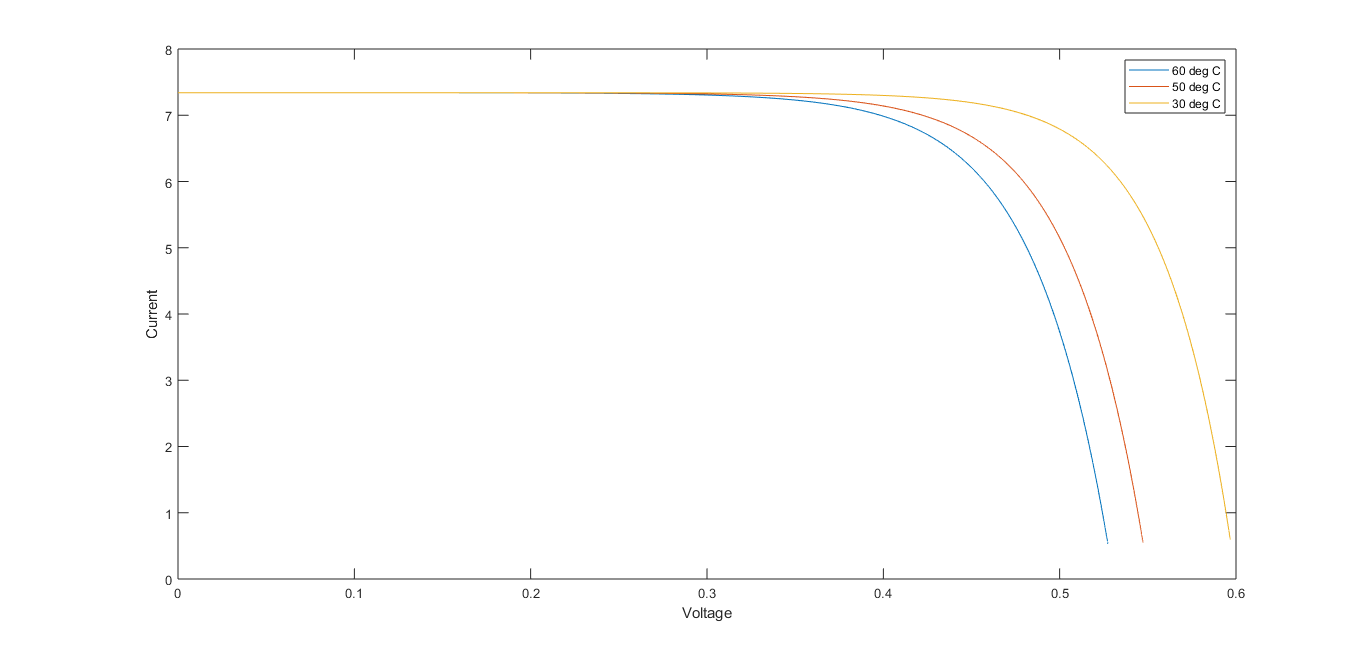
\includegraphics[width=16cm,height=9cm]{I-V for diff temp(1).png}
    \caption{I-V characterstics for different value of temperature.}
    \label{fig:2.7}
\end{figure}



\chapter{Inverter}\label{chap:inverter}

In the middle of 19$^{th}$ to 20$^{th}$ century , the direct current (dc) was converted to alternating current (ac) with the help of motor generator sets (MG sets) and rotary converters. Vacuum tubes as well as gas-filled tubes were used as switches in inverter circuits in the early 20th century \textcolor{blue}{\cite{*_2019}}. An inverter can be defined as device which converts the DC to AC voltage. The inverter is a fixed piece of equipment. It has the ability to transform one type of electrical power into another. However, it is unable to create electricity. As a result, the inverter is a converter rather than a generator. Inverter plays a very crucial role in human's life. For example, a house has a number of equipment which works on 230V AC supply. When the electricity goes off, then the power supply can be provided using an Inverter and a battery system or an Inverter and PV module system or a mixture of both, i.e., it may be used as a stand-alone device for solar or backup power for house appliances. 


\section{Working of Inverter}
The basic model of inverter consist of the dc voltage source as input, switches like IGBT, Thyristor, Mosfet etc., control circuit for controlling the gate pulse of the switches. The number of switches, such as IGBT, Thyristor, mosfet, depends on the type of inverter. The very basic model of inverter, the single phase full-bridge circuit is shown in Figure \ref{fig:3.1}. 

\begin{figure}[hbt!]
    \centering
    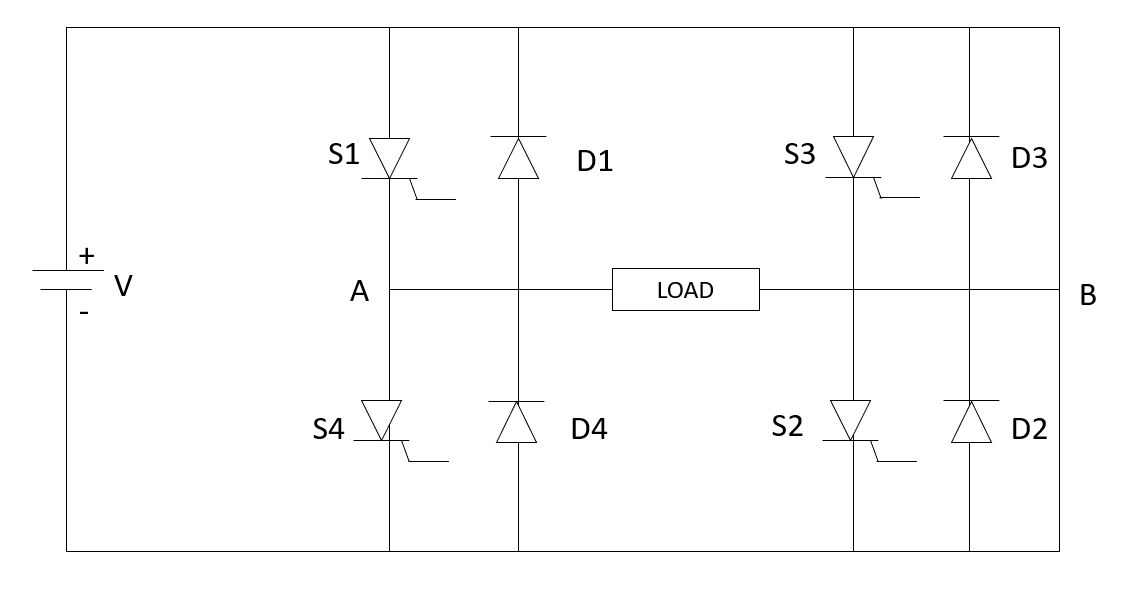
\includegraphics[width = 17.5cm, height = 9cm]{inverter.png}  
    \caption{Single phase Full-bridge inverter}
    \label{fig:3.1}
\end{figure}

\begin{figure}[hbt!]
    \centering
    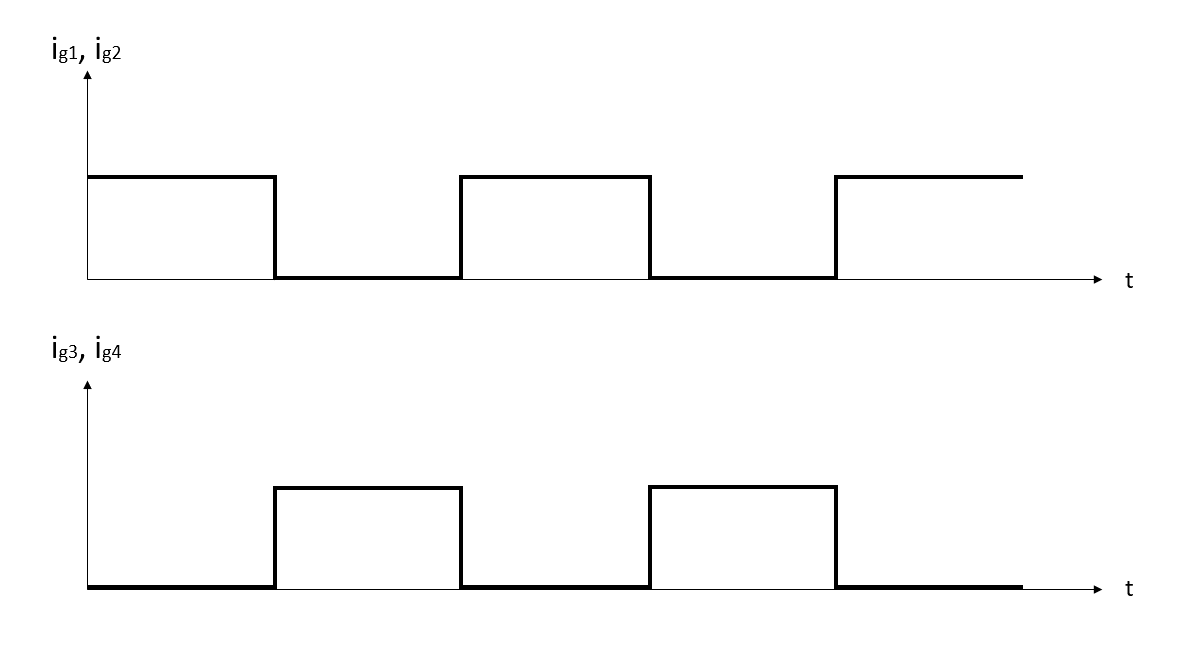
\includegraphics[width = 15cm, height = 8cm]{gate pusle.png}
    \caption{Gate pulse for stitches in inverter}
    \label{fig:3.2}
\end{figure}

\begin{figure}[hbt!]
    \centering
    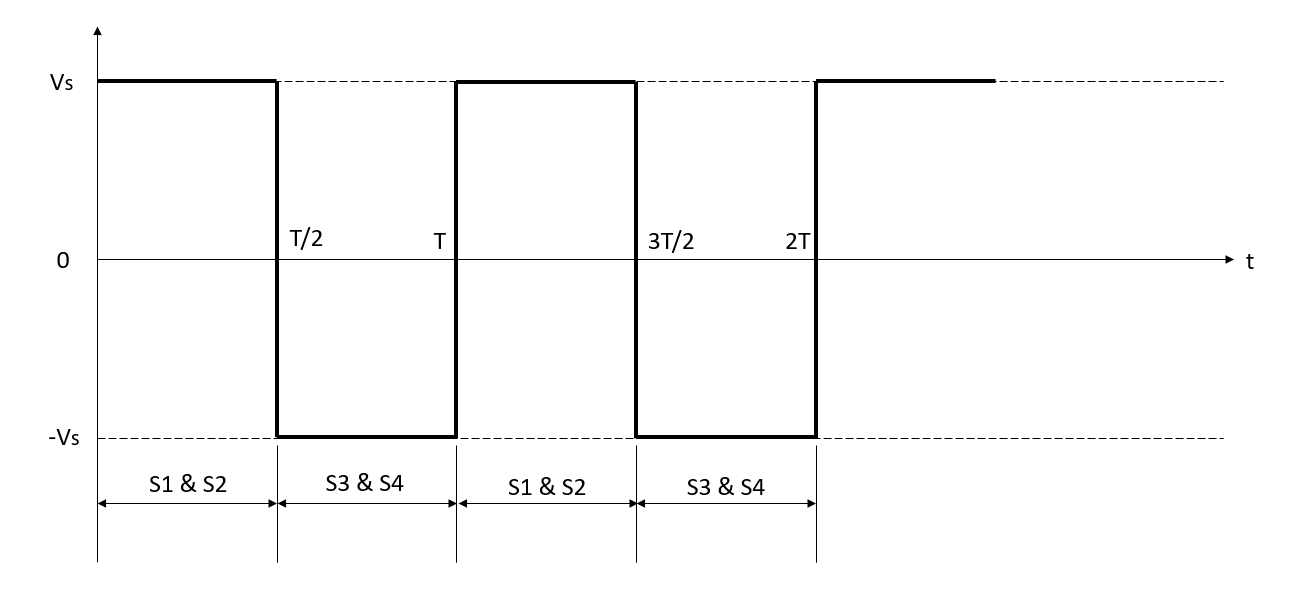
\includegraphics[width = 15cm, height = 8cm]{Output_inv.png}
    \caption{Full-bridge inverter output}
    \label{Inverter output}
\end{figure}


The diodes connected anti-parallel to the switches are called flyback diodes. There is no need to connect diode D1, D2, D3, D4, if the load is fully resistive since the output voltage and current are always in phase. However, for non-purely resistive loads, the load current ($i_o$) will not be in phase with the load voltage ($V_o$). When the main switch is switched off, the diode linked in anti-parallel with the switch will enable current to flow. When these diodes conduct, the energy is transmitted back to the DC source, which is why they are known as flyback diodes (D1, D2, D3, D4).

The successive triggering of switches set diagonally opposite is the operating concept of a single phase full bridge inverter, most commonly thyristor is used as a switching device. This indicates that switches T3 and T4 will be triggered for half of the time period, while T1 and T2 will be triggered for the other half. In half of the time, just two switches are switched on.

Gate pulse waveform is seen in Figure \ref{fig:3.2}. It is observed that switches S1 and S2 are activated at the same moment for a period of time T/2. As a result of S1 and S2 connecting the load to the source, the load voltage is equal to the source voltage with positive polarity. This is why the load voltage in the output voltage waveform is positive and equal to Vs.

S1 and S2 are switched off as soon as the gate signals ($i_{g1}$ and $i_{g2}$) are withdrawn. Consequently, S3 and S4 are switched on at the same time as gate signals ($i_{g3}$ and $i_{g4}$) are applied. The load is linked to the source while S3 and S4 are conducting. The load voltage is again Vs, but this time with opposite polarity. The output voltage is presented as negative in the voltage waveform because of this.

In conclusion, Switches S1 and S2 conduct for the duration $0 < t \leq T/2$ , and the load voltage Vo = Vs. Switches S3 and S4 conduct for time $T/2 < t \leq T$, and load voltage Vo = -Vs.

\section{Types of Solar PV Inverter}

A solar inverter, also known as a PV inverter, is an electrical converter that converts a photovoltaic (PV) solar panel's variable direct current (DC) output into a alternating current (AC)  with a particular frequency that can be fed into a electrical grid or used by a local user. Maximum power point tracking and anti-islanding prevention are two features that solar power converters have developed for use with photovoltaic arrays. The following are the several types of inverters:
\begin{enumerate}
    \item \textbf{Off-Grid Inverters} : Off-grid inverters, which are sometimes also called stand-alone inverters, do not require that a solar panel be connected to them. Instead, they get DC power from batteries that are charged by solar panels or other sources including motor generators, hydro turbines, and wind turbines. Anti-islanding protection is not required as these inverters are separated from utility grids. Furthermore, they are unable to feed extra solar energy to the grid. In isolated places or when individuals prefer to live fully off the grid, off-grid inverters are useful \textcolor{blue}{\cite{oorjanblog_2018}}.
    \item \textbf{Grid Tied Inverters} :Grid-tied inverters are hooked to the utility grid and operate by matching their frequency to that of the sine wave on the utility grid. For safety concerns, they are intended to shut down automatically in the case of a power outage. As a result, they are unable to provide electricity during a blackout. Central plant inverter systems, string inverter systems, multi-string inverter systems, and micro grid inverter (AC modules) systems are the four types of grid-integrated solar PV inverters available today \textcolor{blue}{\cite{oorjanblog_2018}}.
    \item \textbf{Battery-Hybrid Inverters} : These are a hybrid of the previous two inverters, allowing one to be mainly self-sufficient while still being able to connect to the grid in the event of low solar or heavy usage days. Inverters of this type often charge the coupled with a battery first, then export any extra power to the grid. Similarly, during nights/cloudy days, these inverters are adaptive enough to utilise the stored power for consumption first, then recharge the battery via the grid when a specific criterion has been reached. They must be equipped with anti-islanding protection due to grid-syncing. These are an excellent alternative for Indian consumers, but many utilities are reluctant to provide a net-metering connectivity to these hybrid inverters, and the legislation around them are opaque \textcolor{blue}{\cite{oorjanblog_2018}}.
    \item \textbf{String Inverters} : 
    This is the most typical solar inverter for clients, such as Household and commercial users.  These are directly linked to the grid and, in most cases, do not have a backup battery. They're high performance inverters with a 25-year design life and a 5-year guarantee, on average. The best inverters convert DC to AC at a rate of 97–99 percent. On the ground, the less advanced ones will only convert roughly 90-92 percent. Typically, the price and ease of maintenance differences are mirrored in the performance difference \textcolor{blue}{\cite{oorjanblog_2018}}.
    \item \textbf{Micro Inverter} : Microinverters are smaller than ordinary string inverters in terms of size and capacity. For residential applications, the latter is often between 1.5 and 5kW, while the former is often between 200 and 350W. These, unlike string inverters, do not require an array of panels to convert DC. These are mounted on the back of each panel and are in charge of converting the panel to which they are attached. These are a little more expensive, but they're excellent for regions with partial shadowing. These are also known as grid-connected or on-grid inverters \textcolor{blue}{\cite{oorjanblog_2018}}.
    \item \textbf{Central Inverter} : Inverters like this are frequently seen in MW-scale facilities. They're enormous, with their own quarters, exhaust, and so on. They are extremely efficient and contain a lot more grid-related functionality, such as balancing and fluctuation control. Unlike string inverters, they normally start at 400KW \textcolor{blue}{\cite{oorjanblog_2018}}.
\end{enumerate}

\section{MPPT}
A solar cell can operate over a wide range of voltage and current. A monocrystalline silicon solar cell at a temperature of 25$^\circ$Celcius may produce 0.60 volts open circuit voltage ($V_{oc}$). On a full sunny day the cell temperature will probably be close to 45$^\circ$Celcius even though the air temperature is 25$^\circ$Celcius thus reducing the output of solar cell to 0.55 volts per cell. Maximum power is generally produced with 75-80 \% of open circuit voltage ($V_{oc}$) and approximately 90 \% of the short circuit current \textcolor{blue}{\cite{kamil2010grid}}. The maximum power is obtained by tracking the maximum power point by the help of maximum power point tracker (MPPT). The MPPT, based on the output current and voltage of solar cell tracks the maximum power point.    

\section{Methods to establish MPPT}
There are various methods to develop MPPT algorithms. Every method has its own advantage and its disadvantage. These methods are listed below as:

\begin{enumerate}
    \item \textbf{Peturbation and observation (P\&O) method}:
    
    The algorithm for this method is shown in Figure \ref{fig:3.4}. This method compares the output power of the solar cell with the previous sample value. The advantage of P\&O algorithm is its simple nature of algorithm. If the solar radiation does not deviate at a fast rate then the results provided by this method are appropriate \textcolor{blue}{\cite{al2018review}}.
    
    \begin{figure}[hbt!]
        \centering
        \tikzstyle{block}=[draw,rectangle,rounded corners,minimum width=10.5mm,text centered,minimum height=10mm]
        \tikzstyle{block1}=[draw,rectangle,rounded corners,text width=10em,text centered]
        \tikzstyle{arrow} = [thick,->,>=stealth]
        \begin{tikzpicture}
        \centering
        \node[block](bd1){Start};
        \node[block,below
        of=bd1,yshift=-8mm](bd2){Sense V(n), I(n)};
        \node[block,below
        of=bd2,yshift=-8mm](bd3){P(n)-P(n-1)=0};
        \node[block,below
        of=bd3,yshift=-8mm](bd4){P(n)-P(n-1)$>$0};
        \node[block,below
        of=bd4,yshift=-8mm,xshift=33mm](bd5){V(n)-V(n-1)$>$0};
        \node[block,below
        of=bd4,yshift=-7.8mm,xshift=-33mm](bd6){V(n)-V(n-1)$<$0};
        \node[block,below
        of=bd5,yshift=-7.8mm,xshift=-18mm](bd7){Decrease Vref};
        \node[block,below
        of=bd5,yshift=-7.8mm,xshift=19mm](bd8){Increase Vref};
        \node[block,below
        of=bd6,yshift=-7.8mm,xshift=-19mm](bd9){Increase Vref};
        \node[block,below
        of=bd6,yshift=-7.8mm,xshift=19mm](bd10){Decrease Vref};
        \node[block1,below
        of=bd10,yshift=-11mm,xshift=17mm](bd11){V(n-1)=V(n)\\P(n-1)=P(n)};
        \draw[arrow](bd1)->(bd2);
        \draw[arrow](bd2)->(bd3);
        \draw[arrow](bd3)->node[anchor=east]{No}(bd4);
        \draw[arrow](bd4)-|node[anchor=south]{Yes}(bd5);
        \draw[arrow](bd4)-|node[anchor=south]{No}(bd6);
        \draw[arrow](bd5)-|node[anchor=south]{Yes}(bd8);
        \draw[arrow](bd5)-|node[anchor=south]{No}(bd7);
        \draw[arrow](bd6)-|node[anchor=south]{Yes}(bd10);
        \draw[arrow](bd6)-|node[anchor=south]{No}(bd9);
        \draw[arrow](bd11)--node[anchor=south]{Return}(7,-11.03)--(7,-3.6)--(bd3);
        \draw[arrow](bd7)--(1.5,-10);
        \draw[arrow](bd8)--(5.2,-10);
        \draw[arrow](bd9)--(-5.2,-10);
        \draw[arrow](bd10)--(-1.4,-10);
        \draw (-7,-10)--(5.2,-10);
        \draw[arrow](0.3,-10)--(bd11);
        \draw[arrow](bd3)--node[anchor=south]{Yes}(-7,-3.6)--(-7,-10);
        \end{tikzpicture}
        \caption{P\&O method algorithm}
        \label{fig:3.4}
    \end{figure}
    \item \textbf{Incremental Conductance method}
    
    The algorithm for incremental conductance is shown in Figure \ref{fig:3.5}. This method works if dP/dV is equal to zero because at maximum power point (MPP) the derivative of power is zero, if dP/dV is greater than zero it results in the left area of MPP curve and if dP/dV is less than zero it results in the right area of MPP curve. dP/dV can also be expressed as:
    
    \begin{equation}
        \frac{dP}{dV}=\frac{dIV}{dV}\cong I+V\frac{\triangle I}{\triangle V}
    \end{equation}
    
    For MPP, putting $\frac{dP}{dV}=0$, gives
    
    \begin{equation}
        I+V\frac{\triangle I}{\triangle V}=0
    \end{equation}
    
    In extremely variable condition this algorithm works more accurately and it oscillates very less around MPP as compared to P\&O method. The only disadvantage is the complexity of this algorithm.
    
    \begin{figure}[hbt!]
        \centering
        \tikzstyle{block}=[draw,rectangle,rounded corners,minimum width=10.5mm,text centered,minimum height=10mm]
        \tikzstyle{block1}=[draw,rectangle,rounded corners,text width=10em,text centered]
        \tikzstyle{arrow} = [thick,->,>=stealth]
        \begin{tikzpicture}
        \centering
        \node[block](bd1){Start};
        \node[block1,below
        of=bd1,yshift=-8mm](bd2){Sense V(n), I(n)\\$\triangle V=V(n)-V(n-1)$\\$\triangle I=I(n)-I(n-1)$};
        \node[block,below
        of=bd2,yshift=-8mm](bd3){$\triangle V=0$};
        \node[block,below
        of=bd3,yshift=-8mm](bd4){I+($\triangle I/\triangle V)V=0$};
        \node[block,below
        of=bd4,yshift=-8mm](bd5){I+($\triangle I/\triangle V)V>0$};
        \node[block,below
        of=bd5,yshift=-8mm](bd6){Decrease Vref};
        \node[block,left
        of=bd6,xshift=-22mm](bd7){Increase Vref};
        \node[block,right
        of=bd4,xshift=28mm](bd8){$\triangle I=0$};
        \node[block,below
        of=bd8,yshift=-8mm](bd9){$\triangle I>0$};
        \node[block,below
        of=bd9,yshift=-8mm](bd10){Increase Vref};
        \node[block,right
        of=bd10,xshift=22mm](bd11){Decrease Vref};
        \node[block1,below
        of=bd6,yshift=-10mm,xshift=15mm](bd12){V(n-1)=V(n)\\P(n-1)=P(n)};
        
        \draw[arrow](bd1)--(bd2);
        \draw[arrow](bd2)--(bd3);
        \draw[arrow](bd3)--node[anchor=east]{No}(bd4);
        \draw[arrow](bd3)-|node[anchor=south]{Yes}(bd8);
        \draw[arrow](bd8)--node[anchor=east]{No}(bd9);
        \draw[arrow](bd9)--node[anchor=east]{No}(bd10);
        \draw[arrow](bd9)-|node[anchor=south]{Yes}(bd11);
        \draw[arrow](bd5)--node[anchor=east]{No}(bd6);
        \draw[arrow](bd5)-|node[anchor=south]{Yes}(bd7);
        \draw[arrow](bd4)--node[anchor=east]{No}(bd5);
        \draw[arrow](bd7)--(-3.2,-10);
        \draw[arrow](bd6)--(0,-10);
        \draw[arrow](bd10)--(3.8,-10);
        \draw[arrow](bd11)--(7,-10);
        \draw(-5,-10)--(8.7,-10);
        \draw[arrow](1.5,-10)--(bd12);
        \draw[arrow](bd4)--node[anchor=south]{Yes}(-5,-5.4)--(-5,-10);
        \draw[arrow](bd8)--node[anchor=south]{Yes}(8.7,-5.4)--(8.7,-10);
        \draw[arrow](bd12)--node[anchor=south]{Return}(-5.6,-11)--(-5.6,-3.6)--(bd3);
        \end{tikzpicture}
        \caption{Incremental Conductance method algorithm}
    \label{fig:3.5}
    \end{figure}
    
    \item \textbf{Constant Voltage method}
    
    It is one of the simplest algorithm for making MPPT. This method cannot practically find MPP because in this method the operating point is fixed approximately equal to the MPP by setting solar's output voltage. Vref is then regulated to the voltage corresponding to maximum power point Vmpp. This method recquires pre collection of data for a constant Vref \textcolor{blue}{\cite{al2018review}}.
    
    \item \textbf{Fractional Open-Circuit Voltage (FOCV) method}
    
    In this method MPP is calculated using the equation given below:
    
    Let voltage at maximum power point be $V_{max}$ then,
    
    \begin{equation}
        V_{max}\approx M_{oc}*V_{oc}
    \end{equation}
    
    where $M_{oc}$ takes value in the range of 0.78-0.92 and its value can be obtained by a detailed analysis of irradiation and temperature values. In this method the load side is open circuited for a very small time and voltage $V_{oc}$ is measured and then by using the above equation the $V_{max}$ is calculated. This method is easy to implement but it can never attain MPP \textcolor{blue}{\cite{al2018review}}
    
    
\end{enumerate}

\section{MATLAB Simulink model of Inverter}

The simulnk model of the inverter is shown in Figure \ref{fig:3.6} and the output of this inverter is shown in the Figure \ref{fig:3.7}. MPPT is prepared using the P\&O method which generates the gate pulse for the DC-DC boost converter. The DC-AC Converter works on the basis of pulse width mofulation (PWM) technique.

\begin{figure}[hbt!]
    \centering
    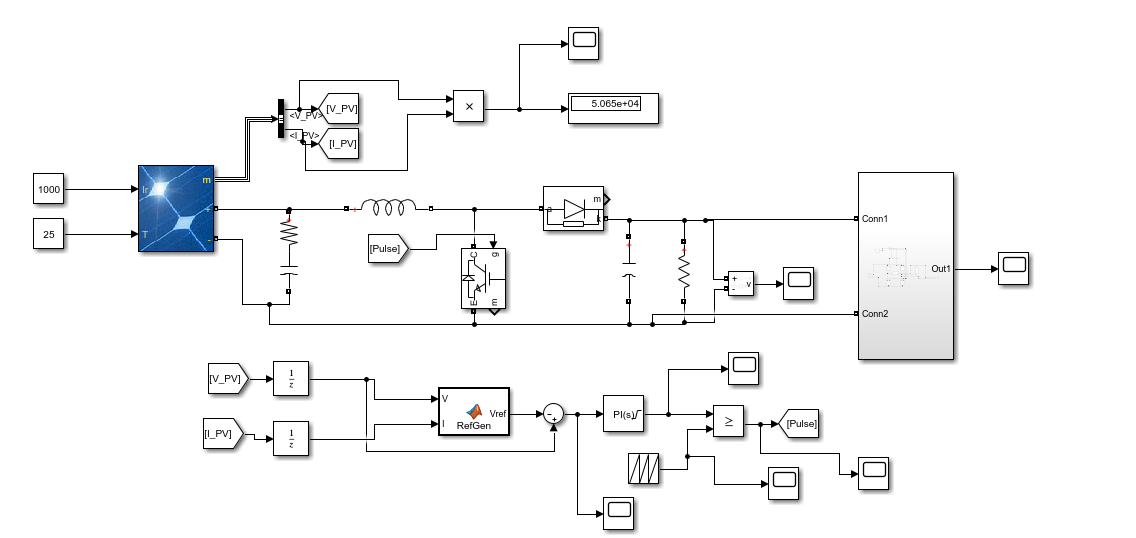
\includegraphics[width=18cm,height=10cm]{Final DC_DC_AC(1).png}
    \caption{Final model of Inverter}
    \label{fig:3.6}
\end{figure}

\begin{figure}[hbt!]
    \centering
    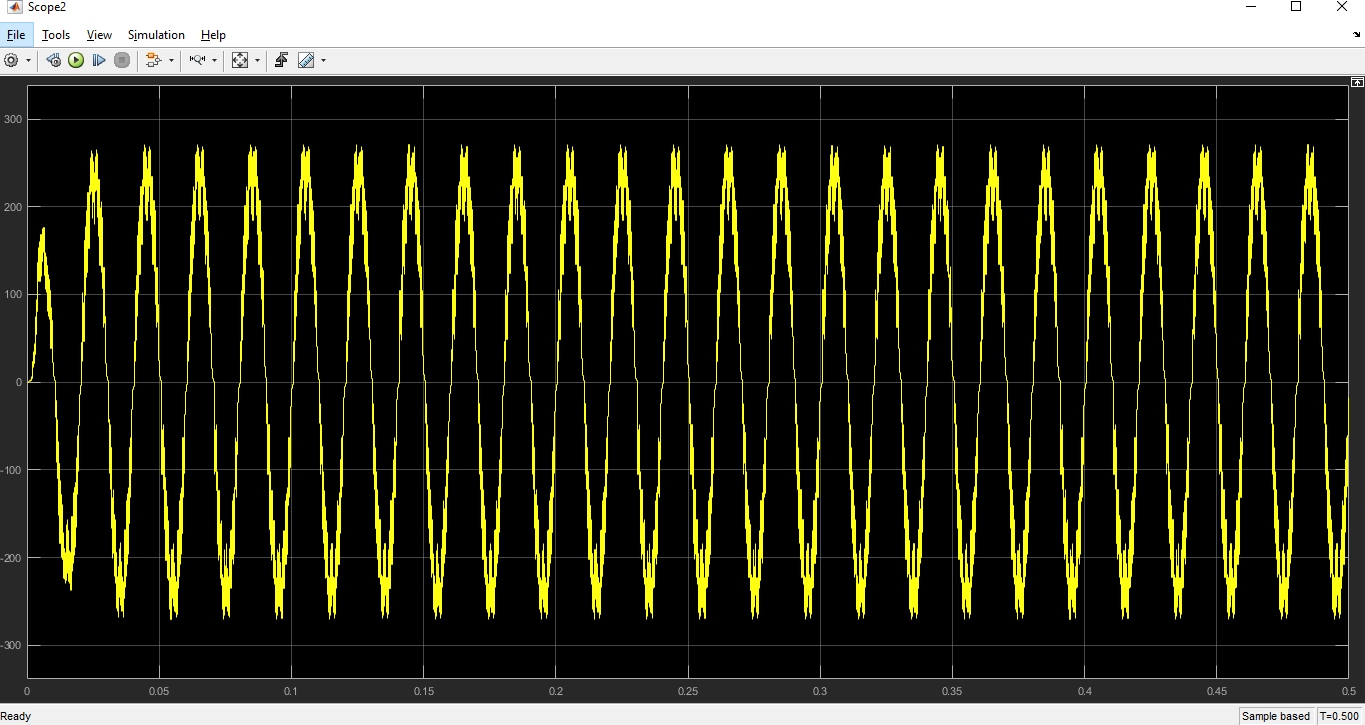
\includegraphics[width=15.8cm,height=10cm]{Final result DC-AC(1).png}
    \caption{Output of Inverter}
    \label{fig:3.7}
\end{figure}

\chapter{Controller Part of Inverter}\label{chap: Controller Part of Inverter}
\section{STM32F407VG Discovery Board}
This discovery board is based on STM32F407VGT6 and has an inbuilt ST-Link/V2 debug tool interface, ST MEMS digital microphone, ST MEMS digital accelerometer, LEDs, push buttons, audio DAC with integrated class D speaker driver, USB OTG micro-AB connector. The discovery board is shown in the Figure \ref{fig:4.1}. It is a low-cost device \textcolor{blue}{\cite{um14722012stm32f4discovery}}. The development tool chain that supports the STM discovery board are
\begin{enumerate}
    \item Altium, Tasking VX Toolset
    \item Atollic True studio
    \item IAR, EWARM
    \item Keil, MDK-ARM
\end{enumerate}
It has following features:
\begin{enumerate}
    \item Two Push buttons.
    \begin{itemize}
        \item B1 User: Connected to PA0 of microcontroller. It is blue in colour.
        \item B2 Reset: It is connected to NRST and resets the microcontroller. It is black in colour.
    \end{itemize}
    \item Eight LEDs each for different purpose.
    \begin{itemize}
    \item LD1 COM: It's default status is red. It turns green to show the communication is happening between PC and board.
    \item LD2 PWR: It shows red colour which means that the board is getting power.
    \item User LD3: It is an orange LED connected to pin PD13 of the microcontroller.
    \item User LD4: It's a green LED conected to PD12 of microcontroller.
    \item User LD5: It's a red LED connected to PD14 of microcontroller
    \item User LD6: It's a blue LED connected to PD15 of microcontroller.
    \item USB LD7: It's a green LED connected to PA9 of microcontroller which indicates the presence of VBUS on CN5.
    \item USB LD8: It's a red LED that is connected to PD5 of microcontroller that shows the overcurrent from VBUS of CN5.
    \end{itemize}
    \item It has 1MB of flash memory and 192 KB of RAM in a LQFP100 Package.
    \end{enumerate}
This discovery board is designed with the STM32F407VGT6 microcontroller in a 100-pin LQFP package. This microcontroller is a ARM Cortex-M4 32-bit unit with FPU having 210 DMIPS. The microcontroller is shown in Figure \ref{fig:4.2}. The power supply is provided either by the PC which is connected to discovery board through a USB cable or by an external supply of 5V.


\begin{figure}[hbt!]
    \centering
    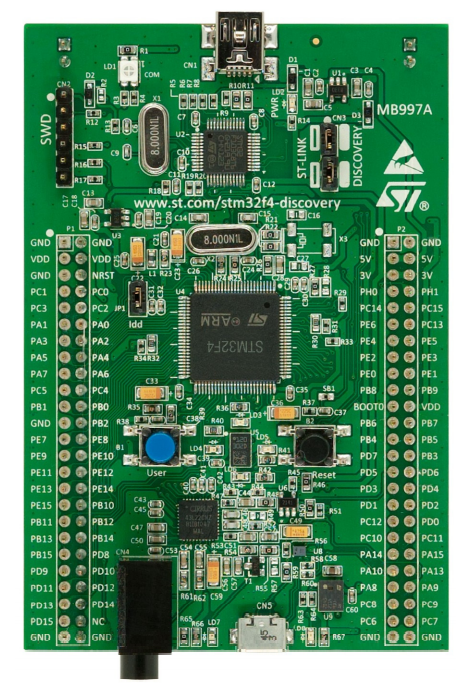
\includegraphics[height=9cm]{STM board.png}
    \caption{STM Discovery Board (adapted from \textcolor{blue}{\cite{um14722012stm32f4discovery}})}
    \label{fig:4.1}
\end{figure}

\begin{figure}[hbt!]
    \centering
    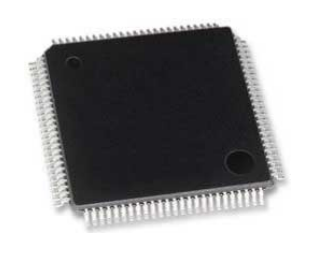
\includegraphics[width=8cm,height=5cm]{microcontroller.png}
    \caption{STM32F407VGT6 Micro-controller (adapted from \textcolor{blue}{\cite{um14722012stm32f4discovery}})}
    \label{fig:4.2}
\end{figure}

\section{Waijung Blockset}
It is a simulink blockset or a library in simulink which makes it easier for generating a C code from the simulink model for a number of microcontrollers. This library currently provides a path to support the generation of C codes for STM32F4 microcontrollers. It supports all the microcontrollers that belong to the family of STM32F4 \textcolor{blue}{\cite{waijungblockset}}.

\section{Proposed Plan}
As this project aimed towards making a hybrid model of inverter system that would behave as an On-grid and Off-grid system depending on the availability of the electricity supply from the grid, there was a need to have a control strategy that would regulate the working of hybrid system. Therefore a flow strategy of the controller part is thought and is shown in Figure \ref{fig:4.1}.

In the Figure \ref{fig:4.1} we can see that PV module gets the sun rays from the sun and it converts the solar energy into electrical energy. This DC form of energy from PV module is fed to DC-DC Boost converter which further goes to DC-AC converter to get AC form of electric energy. The output of DC-AC converter has three paths to flow as shown in figure \ref{fig:4.1}, the paths are:

1) Path (P1) : From DC-AC converter to Grid.

2) Path (P2) : From DC-AC converter to household load.

3) Path (P3) : From DC-AC converter to battery system via AC-DC converter.

The path P4 takes output of PV module and based on it controls the output of DC-DC converter so that the hybrid model works at maximum power point (MPP).

Motive was to regulate the working of hybrid system by controlling the closing and opening of these path (P1, P2, P3) based on whether the grid supply is there or not. The plan states that if grid supply is on then the path P1 will be closed i.e.. the power from DC-AC converter will go directly to the grid while path P2, P3 will be Open. On the other hand if grid supply is Off then the path P1 will be open and path P2 will be closed i.e.. the power from DC-AC converter will be fed to household load. The path P3 will get closed depending on the state of charge of battery i.e.. if battery is uncharged or low charged then the path P3 will get closed. The path P4 will always remain closed to ensure system works at MPP.


\newpage
\begin{figure}[hbt!]
\centering
\tikzstyle{block}=[draw,rectangle,rounded corners,minimum width=5mm,text centered,minimum height=14mm]
\tikzstyle{block1}=[draw,rectangle,rounded corners,text width=5em,text centered]
\tikzstyle{arrow} = [thick,->,>=stealth]

\begin{tikzpicture}
\centering
\node[block](bd1){PV module};
\node[block1,right
of=bd1,xshift=25mm](bd2){DC-DC Boost Converter};
\node[block1,right
of=bd2,xshift=25mm](bd3){DC-AC Converter};
\node[block1,right
of=bd3,xshift=25mm](bd4){Grid};
\node[block1,below
of=bd4,yshift=-10mm](bd5){Household Load};
\node[block1,below
of=bd5,yshift=-10mm](bd6){Battery System};
\node[block1,below
of=bd3,yshift=-30.5mm](bd7){AC-DC Converter};
\node[block1,above
of=bd3,yshift=18mm](bd8){PLL};
\node[block1,below
of=bd1,yshift=-32.2mm](bd9){MPPT};
\node[block1,above
of=bd1,yshift=18mm](bd10){Sun Rays};
\draw[arrow](bd1)->(bd2);
\draw[arrow](bd2)->(bd3);
\draw[arrow](bd3)--node[anchor=south]{\textcolor{green}{P1}}(bd4);
\draw[arrow](bd3)--node[anchor=south]{\textcolor{green}{P2}}(bd5);
\draw[arrow](bd3)--node[anchor=east]{\textcolor{green}{P3}}(bd7);
\draw[arrow](bd7)->(bd6);
\draw[arrow](bd1)--node[anchor=west]{\textcolor{green}{P4}}(bd9);
\draw[arrow](bd9)-|(bd2);
\draw[arrow](bd10)->(bd1);
\draw[arrow](bd4)|-(bd8);
\draw[arrow](bd8)--(bd3);
\end{tikzpicture}
\caption{Flow Diagram of our proposed plan for Hybrid Inverter System}
\label{fig:4.3}
\end{figure}

\section{Proposed method}

    STM32F407VG discovery board is used here for implementing these control strategies. Help of waijung blookset \textcolor{blue}{\cite{waijungblockset}} and STM coding using Atollic true studio for STM32 \textcolor{blue}{\cite{stmicroelectronics}} is taken for the same. Flow diagram for the proposed method is shown in Figure \ref{fig:4.4}

The inputs to the micro controller are from the grid via voltage sensing circuit, voltage and curent of pv module through sensing circuit. The STM board is shown in Figure \ref{fig:4.5} with the inputs and outputs. 

\newpage
\begin{figure}[hbt!]
\centering
\tikzstyle{block}=[draw,rectangle,rounded corners,minimum width=5mm,text centered,minimum height=14mm]
\tikzstyle{block1}=[draw,rectangle,rounded corners,text width=5em,text centered]
\tikzstyle{block2}=[draw=black,rectangle,rounded corners,text width=5em,text centered,fill=red!30]
\tikzstyle{block3}=[draw=black,rectangle,rounded corners,text width=5em,text centered,fill=blue!30]
\tikzstyle{block4}=[draw=black,rectangle,rounded corners,text width=5em,text centered,fill=green!30]
\tikzstyle{block5}=[draw=black,rectangle,rounded corners,text width=5em,text centered,fill=orange!30]
\tikzstyle{block6}=[draw=black,rectangle,rounded corners,text width=5em,text centered,fill=cyan!30]
\tikzstyle{block7}=[draw=black,rectangle,rounded corners,text width=5em,text centered,fill=yellow!30]
\tikzstyle{block8}=[draw=black,rectangle,rounded corners,text width=5em,text centered,fill=pink!30]
\tikzstyle{arrow} = [thick,->,>=stealth]
\begin{tikzpicture}
\centering
\node[block1](bd1){Sun Rays};
\node[block1,below
of=bd1,yshift=-10mm](bd2){PV Module};
\node[block1,right
of=bd2,xshift=20mm](bd3){DC-DC Boost Converter};
\node[block1,right
of=bd3,xshift=20mm](bd4){DC-AC Converter};
\node[block1,right
of=bd4,xshift=20mm](bd5){Relay Switch 1};
\node[block1,right
of=bd5,xshift=20mm](bd6){Grid};
\node[block1,below
of=bd6,yshift=-19mm](bd7){Voltage sensing circuit};
\node[block2,below
of=bd7,yshift=-22mm](bd8){V of Grid};
\node[block1,below
of=bd2,yshift=-33mm](bd9){Sensing Circuit};
\node[block6,below
of=bd9,yshift=-10mm](bd10){V of PV};
\node[block7,right
of=bd10,xshift=19mm](bd11){I of PV};
\node[block3,below
of=bd5,yshift=-10mm](bd12){On/off command R1};
\node[block1,below
of=bd4,yshift=-19mm](bd13){Relay Switch 2};
\node[block4,left
of=bd13,xshift=-19mm](bd14){On/off Command R2};
\node[block1,below
of=bd13,yshift=-21mm](bd15){Household Load};
\node[block1,above
of=bd4,yshift=19mm](bd16){Relay Switch 3};
\node[block1,above
of=bd16,yshift=10mm](bd17){AC-DC Converter};
\node[block1,right
of=bd17,xshift=19mm](bd18){Battery System};
\node[block5,right
of=bd16,xshift=19mm](bd19){On/off Command R3};
\node[block8,above
of=bd3,yshift=10mm](bd20){Gate Pulse};
\draw[arrow](bd13)->(bd15);
\draw[arrow](bd4)->(bd13);
\draw[arrow](bd14)->(bd13);
\draw[arrow](bd12)->(bd5);
\draw[arrow](bd1)->(bd2);
\draw[arrow](bd2)->(bd3);
\draw[arrow](bd3)->(bd4);
\draw[arrow](bd4)->(bd5);
\draw[arrow](bd5)->(bd6);
\draw[arrow](bd6)->(bd7);
\draw[arrow](bd7)->(bd8);
\draw[arrow](bd2)->(bd9);
\draw[arrow](bd9)->(bd10);
\draw[arrow](bd9)-|(bd11);
\draw[arrow](bd4)->(bd16);
\draw[arrow](bd16)->(bd17);
\draw[arrow](bd17)->(bd18);
\draw[arrow](bd19)->(bd16);
\draw[arrow](bd20)->(bd3);
\end{tikzpicture}
\caption{Flow Diagram of our proposed method for Hybrid Inverter System}
\label{fig:4.4}
\end{figure}


\begin{figure}[hbt!]
\centering
\tikzstyle{block}=[draw,rectangle,rounded corners,minimum width=5mm,text centered,minimum height=14mm]
\tikzstyle{block1}=[draw,rectangle,rounded corners,text width=5em,text centered]
\tikzstyle{block2}=[draw=black,rectangle,rounded corners,text width=5em,text centered,fill=red!30]
\tikzstyle{block3}=[draw=black,rectangle,rounded corners,text width=5em,text centered,fill=blue!30]
\tikzstyle{block4}=[draw=black,rectangle,rounded corners,text width=5em,text centered,fill=green!30]
\tikzstyle{block5}=[draw=black,rectangle,rounded corners,text width=5em,text centered,fill=orange!30]
\tikzstyle{block6}=[draw=black,rectangle,rounded corners,text width=5em,text centered,fill=cyan!30]
\tikzstyle{block7}=[draw=black,rectangle,rounded corners,text width=5em,text centered,fill=yellow!30]
\tikzstyle{block8}=[draw=black,rectangle,rounded corners,text width=5em,text centered,fill=pink!30]
\tikzstyle{arrow} = [thick,->,>=stealth]
\begin{tikzpicture}
\centering
\node[block1](bd1){STM Discovery Board};
\node[block2,left
of=bd1,xshift=-30mm,yshift=11mm](bd2){V of Grid};
\node[block6,left
of=bd1,xshift=-30mm](bd3){V of PV};
\node[block7,left
of=bd1,xshift=-30mm,yshift=-11mm](bd4){I of PV};
\node[block3,right
of=bd1,xshift=30mm,yshift=11mm](bd5){On/off command R1};
\node[block4,left
of=bd1,xshift=50mm,yshift=-10mm](bd6){On/off Command R2};
\node[block8,right
of=bd1,xshift=30mm,yshift=-40mm](bd8){Gate Pulse};


\draw[arrow](bd1)->(bd6);
\draw[arrow](bd1)->(bd8);
\draw[arrow](bd1)->(bd5);
\draw[arrow](bd2)-|(bd1);
\draw[arrow](bd3)->(bd1);
\draw[arrow](bd4)-|(bd1);
\end{tikzpicture}
\caption{STM Discovery board with input and outputs.}
\label{fig:4.5}
\end{figure}

\section{Methodology}
To begin this project, study of STM32F4 discovery board was done in detail. After getting sufficient background knowledge of STM32F4 discovery board, study on waijung blookset was done in detail and its few pre-built models provided by waijung library were tested on discovery board. The models are shown in Appendix \ref{Models created using Waijung Library}. This Testing was done after the proper connection was established between the STM32 discovery board and the computer. This connection was done by downloading few softwares like ST-Link \textcolor{blue}{\cite{stmicroelectronics1}}, ST-Link\_USB\_V2\_1\_Driver, keil MDK-ARM version for proper running of discovery board. Various models were made using waijung blookset for the controller part for the proposed hybrid system but there were some errors in it and because of which the plan of controlling the path P1, P2, P3 was not satisfied fully.

For path P4, controller (MPPT) was built in MATLAB simulink as shown in Figure \ref{fig:4.6}. It was not made using waijung blookset. After all these attempts new approach was used which was to build codes for STM micro controller and which was done using atollic true studio for STM32. Few basic codes were made in order to understand the STM coding, which are shown in Appendix \ref{STM Demo Codes}. Algorithm for MPPT is shown in Figure \ref{fig:4.9} and the exact code can be seen in Appendix \ref{STM Demo Codes}. Algorithm for controlling the path P1 and P2 is shown in Figure \ref{fig:4.8} and the exact code can be seen in Appendix \ref{STM Demo Codes}. PLL was also prepared which will be discussed later in this report in detail.

For path P3 mentioned in Figure \ref{fig:4.3}, a small simulink model for the same has been thought of which is shown in Figure \ref{fig:4.7}.

\subsection{Working Strategy}
All the codes would be uploaded in the STM discovery board. Relay are the switches that gets closed or open depending on the signal received by it through the signal pin. If the input to the signal pin is high then the relay will get closed and if the input to the signal pin is low then the relay will get open. The code for controlling the opening and closing of path P1 and P2 will take voltage of grid as input labelled as \enquote{V of Grid} as shown in Figure \ref{fig:4.5}. Based on code if the voltage of grid is some positive quantity then the microcontroller will send a high pulse and pass it through variable labelled as \enquote{On/off command R1} and will make the relay switch 1 closed, and if the voltage of grid is zero then the discovery board will generate a high pulse and pass it through variable labelled as \enquote{On/off command R2} and will make the relay switch 2 closed.

For the path P4 mentioned in Figure \ref{fig:4.3}, code is prepared for MPPT mentioned in Figure \ref{fig:4.9}. This code will take voltage and current of PV module as input labelled as \enquote{V of PV} and \enquote{I of PV} as shown in Figure \ref{fig:4.5}. Based on the algorithm it will generate duty cycle for the DC-DC converter and pass it through variable \enquote{Gate Pulse} to the respective converter. The sensing circuit for PV module can be made using an op-amp and few resistors. The voltage is amplified by an op-Amp before being sent to the controller's ADC. Several preset resistors are employed to modify the voltages to 3.3 V before feeding them to the controller \textcolor{blue}{\cite{tamkoriadesign}}.

The simulink model shown in the Figure \ref{fig:4.7} represents the basic idea as to how the relay switch 3 be turned on/off. This model consist of a simple AC-DC converter which converts AC to DC using the fixed gate pulse. The ac voltage source supplies the power to the resistive load and the battery depending on whether the circuit breaker is closed or open. There are two circuit breaker in this model which get closed and open depending on the command given to them via \enquote{LoadOn} and \enquote{ChargingOn} variable. LoadOn and ChargingOn gets the value (1 or 0) based on the algorithm written in the matlab function block. This matlab function block takes the state of charge (SOC) of battery as the input. If the SOC is less than 100 it closes the ChargingOn breaker and opens the LoadOn breaker, but if the SOC is 100 then it closes the LoadOn breaker and opens the ChargingOn breaker.



\begin{figure}[hbt!]
    \centering
    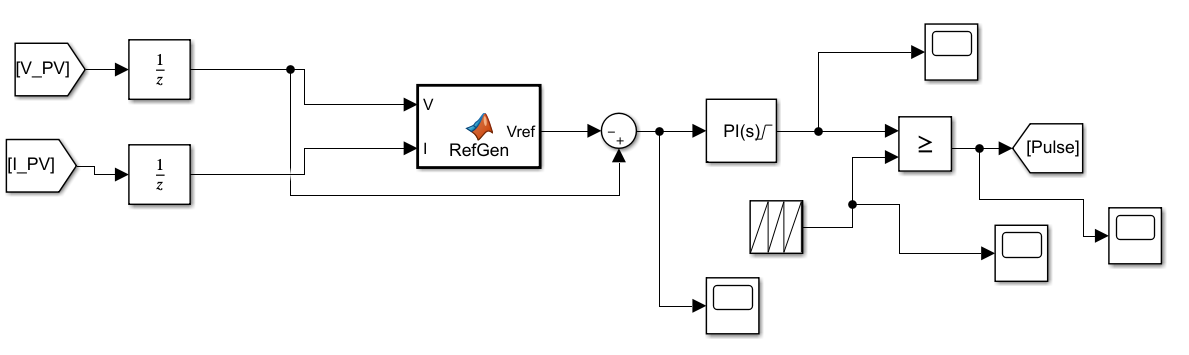
\includegraphics[width=15cm,height=7cm]{MPPT(model simulink).png}
    \caption{Simulink model for MPPT}
    \label{fig:4.6}
\end{figure}

\begin{figure}[hbt!]
    \centering
    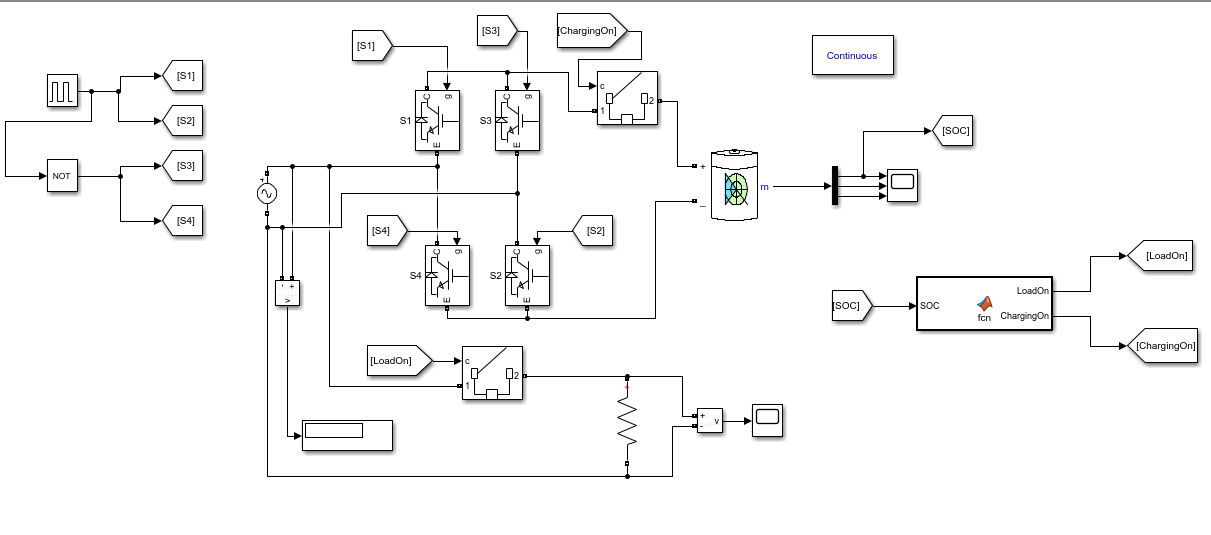
\includegraphics[width=18cm,height=10cm]{path P4.png}
    \caption{Model for path P4.}
    \label{fig:4.7}
\end{figure}

%%%%FLOW CHART FOR CODES%%%%%%%%%%
\begin{figure}[hbt!]
\centering
\tikzstyle{block}=[draw,rectangle,rounded corners,minimum width=5mm,text centered,minimum height=14mm]
\tikzstyle{block1}=[draw,rectangle,rounded corners,text width=5em,text centered]
\tikzstyle{block2}=[draw=black,rectangle,rounded corners,text width=5em,text centered,fill=red!30]
\tikzstyle{block3}=[draw=black,rectangle,rounded corners,text width=5em,text centered,fill=blue!30]
\tikzstyle{block4}=[draw=black,rectangle,rounded corners,text width=5em,text centered,fill=green!30]
\tikzstyle{block5}=[draw=black,rectangle,rounded corners,text width=5em,text centered,fill=orange!30]
\tikzstyle{block6}=[draw=black,rectangle,rounded corners,text width=5em,text centered,fill=cyan!30]
\tikzstyle{block7}=[draw=black,rectangle,rounded corners,text width=5em,text centered,fill=yellow!30]
\tikzstyle{block8}=[draw=black,rectangle,rounded corners,text width=5em,text centered,fill=pink!30]
\tikzstyle{arrow} = [thick,->,>=stealth]
\begin{tikzpicture}
\centering
\node[block](bd1){Include STM Library};
\node[block,below
of=bd1,yshift=-10mm](bd2){Initialize/Declare the function};
\node[block,below
of=bd2,yshift=-10mm](bd3){Begin The main function};
\node[block,below
of=bd3,yshift=-10mm](bd4){Initialize the clock pulse of the port A, D, E};
\node[block,below
of=bd4,yshift=-10mm](bd5){Initialize the pin to be used and call the declared function};
\node[block,below
of=bd5,yshift=-10mm](bd6){Begin a infinite while loop};
\node[block,below
of=bd6,yshift=-10mm](bd7){V of grid $>$ 0};
\node[block1,below
of=bd7,yshift=-10mm,xshift=30mm](bd8){High pulse to Relay switch 1};
\node[block1,below
of=bd7,yshift=-10mm,xshift=-30mm](bd9){High pulse to Relay switch 2};
\draw[arrow](bd1)--(bd2);
\draw[arrow](bd2)--(bd3);
\draw[arrow](bd3)--(bd4);
\draw[arrow](bd4)--(bd5);
\draw[arrow](bd5)--(bd6);
\draw[arrow](bd6)--(bd7);
\draw[arrow](bd7)-|node[anchor=south]{Yes}(bd8);
\draw[arrow](bd7)-|node[anchor=south]{No}(bd9);
\end{tikzpicture}
\caption{Algorithm for Controlling path P1 and P2}
\label{fig:4.8}
\end{figure}

\begin{figure}[hbt!]
        \centering
        \tikzstyle{block}=[draw,rectangle,rounded corners,minimum width=10.5mm,text centered,minimum height=10mm]
        \tikzstyle{block1}=[draw,rectangle,rounded corners,text width=10em,text centered]
        \tikzstyle{arrow} = [thick,->,>=stealth]
        \begin{tikzpicture}
        \centering
        \node[block](bs1){Include STM Library};
        \node[block,below
         of=bs1,yshift=-8mm](bs2){Initialize/Declare the function};
        \node[block,below
         of=bs2,yshift=-8mm](bs3){Begin The main function};
        \node[block,below
         of=bs3,yshift=-8mm](bs4){Initialize the clock pulse of the port to be used};
        \node[block,below 
         of=bs4,yshift=-8mm](bs5){Initialize the pin to be used and call the declared function};
        \node[block,below
         of=bs5,yshift=-8mm](bs6){Begin a infinite while loop} ;
        \node[block,below
        of=bs6,yshift=-8mm](bd2){Sense V(n), I(n)};
        \node[block,below
        of=bd2,yshift=-8mm](bd3){P(n)-P(n-1)=0};
        \node[block,below
        of=bd3,yshift=-8mm](bd4){P(n)-P(n-1)$>$0};
        \node[block,below
        of=bd4,yshift=-8mm,xshift=33mm](bd5){V(n)-V(n-1)$>$0};
        \node[block,below
        of=bd4,yshift=-7.8mm,xshift=-33mm](bd6){V(n)-V(n-1)$<$0};
        \node[block,below
        of=bd5,yshift=-7.8mm,xshift=-18mm](bd7){Decrease Vref};
        \node[block,below
        of=bd5,yshift=-7.8mm,xshift=19mm](bd8){Increase Vref};
        \node[block,below
        of=bd6,yshift=-7.8mm,xshift=-19mm](bd9){Increase Vref};
        \node[block,below
        of=bd6,yshift=-7.8mm,xshift=19mm](bd10){Decrease Vref};
        \node[block1,below
        of=bd10,yshift=-11mm,xshift=17mm](bd11){V(n-1)=V(n)\\P(n-1)=P(n)};
        
        \draw[arrow](bs1)->(bs2);
        \draw[arrow](bs2)->(bs3);
        \draw[arrow](bs3)->(bs4);
        \draw[arrow](bs4)->(bs5);
        \draw[arrow](bs5)->(bs6);
        \draw[arrow](bs6)->(bd2);
        \draw[arrow](bd2)->(bd3);
        \draw[arrow](bd3)->node[anchor=east]{No}(bd4);
        \draw[arrow](bd4)-|node[anchor=south]{Yes}(bd5);
        \draw[arrow](bd4)-|node[anchor=south]{No}(bd6);
        \draw[arrow](bd5)-|node[anchor=south]{Yes}(bd8);
        \draw[arrow](bd5)-|node[anchor=south]{No}(bd7);
        \draw[arrow](bd6)-|node[anchor=south]{Yes}(bd10);
        \draw[arrow](bd6)-|node[anchor=south]{No}(bd9);
        \draw[arrow](bd11)--node[anchor=south]{Return}(7.2,-20.1)--(7.2,-12.6)--(bd3);
        \draw[arrow](bd7)--(1.51,-19);
        \draw[arrow](bd8)--(5.2,-19);
        \draw[arrow](bd9)--(-5.2,-19);
        \draw[arrow](bd10)--(-1.4,-19);
        \draw (-7.2,-19)--(5.2,-19);
        \draw[arrow](0.3,-19)--(bd11);
        \draw[arrow](bd3)--node[anchor=south]{Yes}(-7.2,-12.6)--(-7.2,-19);
        \end{tikzpicture}
        \caption{Algorithm for MPPT.}
        \label{fig:4.9}
    \end{figure}


%%%%%%%%%%%%%%%%%%%%%%%%%%%%%%%%%%%%%%%%%%%%%%%%%%%%%%%%%%%%%%%%%%%%%%%%%%%%%%%%%%SATVIK%%%%%SATVIK%%%%%%%%%%%%%%%%%%%%%%%%%%%%%%%%%%%%%%%%%


\chapter{Inverter-Grid Synchronisation}\label{chap:Inverter-Grid Synchronisation}

Even though renewable energy sources and distributed generation have been employed for more than two decades, there are still certain aspects that need to be improved in order to improve energy distribution and quality in the utility grid to levels needed by various standards and, most importantly, to meet the needs of customers. One of the primary issues in this regard is synchronising the current at the output of the inverter with the voltage of the utility grid \cite{rocabert2012control}.

A grid-connected solar power generating facility must be constantly alert to avoid grid disruptions and must be able to isolate when the system fails. If it does not isolate, the generated solar power will feed the grid, causing the solar plant to become overloaded and could cause injuries to the components inside the converters and other elements.
It is indeed crucial to note that once the grid is disconnected, the solar power will continue to provide power even if work on the power system network is ongoing. 
Even though the grid is isolated, the customer must be receiving power since local loads require continuity, which isolation mode assists with.
As a result, the utility will be separated, and the customer will not have an impact on the supply's continuity. 

The accuracy with which the ac grid voltage parameters are assessed has a significant impact on the overall performance of grid-connected devices. To estimate the grid voltage characteristics, such as voltage amplitude, frequency, and phase angle, a precise synchronisation method is required, as these values are required for accurate synchronisation with the grid and delivery of generated electricity \cite{rocabert2012control}.

\section{Phase Loccked-Loop(PLL)}

 PLL is widely used in signal processing, including radio and telecommunications, computers, and electrical motor control. The approaches can be used across a wide range of frequencies, from a few hertz to orders of gigahertz. 

The output voltage from the inverter must have the same frequency for each of the three phases in order to connect a power plant to the grid. If the phase angle of the grid voltage is tracked, this can be accomplished. This is a real-time procedure that is always running in order to keep the inverter output synchronised with the grid. 

Standard synchronisation methodologies of the inverter current and the grid voltage involve widespread algorithms based on the phase-locked loops (PLL). Because utility voltage is rarely a pure sine wave, the PLL system must be able to manage distortions and irregularities satisfactorily.
Unbalance in the three-phase system, presence of harmonics, variation in frequency, variation in amplitude, and phase leaps are all possible distortions in the grid voltage. These non-ideal situations arise for a variety of reasons. When a load or generator connects or disconnects from the grid, phase jumps and unbalances can occur. Grid voltages may experience harmonics as a result of transformers or devices having non-linear properties \cite{schlabbach2001voltage}.

A PLL tracks one signal by another, and as a result of this tracking, the output signal is phase and frequency synced with the input reference signal. Because of their efficiency and resilience, various PLL approaches have been proposed and are utilised in single-phase, three-phase, and aviation electrical systems \cite{cupertino2010running}, whenever you need to keep track of currents and voltages. In general, Phase Lock Loop is the control loop or the control system which maintains the same phase between the input or the reference signal and the output signal.  

For a long time, the tracing technique has been utilised, investigated, and developed. Different methods to implement the PLL in three-phase and single-phase applications can be found in the following three literature.  Reference \cite{hsieh1996phase} \cite{guo2011phase} \cite{devi2015phase} offers an overview of the phased-locked loops' historical development, general information on their function, and a more extensive study of the three major blocks that make up the overall PLL, these major blocks are shown in figure 5.1. The basic structure of the most widely accepted synchronisation solution for a time-varying signal can be described by the block diagram shown in Fig. 5.1, which summarises the structure of nearly every PLL algorithm currently available in any literature, where the phase angle difference between the input and output signal is measured by phase detection (PD) and passed through the loop filter (LF). The voltage-controlled oscillator (VCO) is driven by the LF output signal to generate the output signal, which could follow the input signal.  

\begin{figure} 
    
    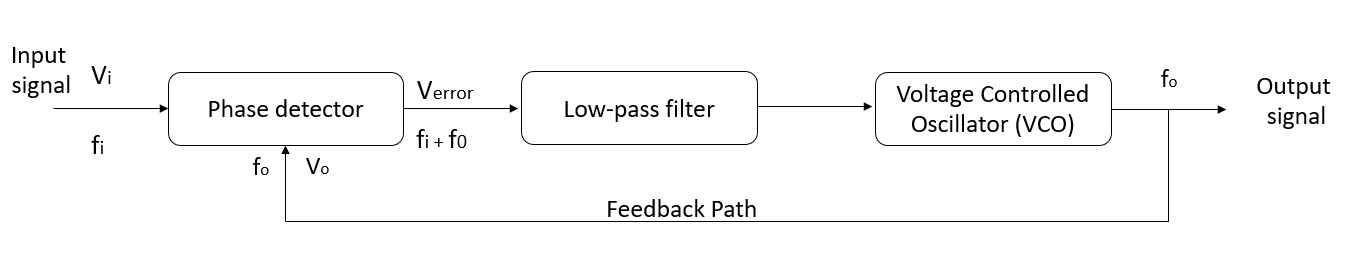
\includegraphics[width=1.0\textwidth]{PLL block diagram.png}
    \caption{PLL Block diagram}
\end{figure}



\subsection{Synchronous Reference Frame PLL (SRF-PLL)}

A number of PLLs have recently been created for three-phase grid-connected power converters, the most common of which is the synchronous reference frame PLL (SRF-PLL) \cite{golestan2012design}. The synchronous-reference frame PLL's fundamental idea is to transform the input signals into dq-frame using the well-known Park and Clark transformations. Reference \cite{golestan2012design} proposes a concept for such a PLL. The Synchronous Rotating Reference Frame PLL (SRF-PLL) is the PLL system that performs best under distorted and non-ideal grid settings \cite{ghoshal2007method}. An adaptive synchronous reference frame PLL is proposed in \cite{gonzalez2011adaptive} in the scenario of grid-inverter operation in a polluted utility grid to improve energy quality.
The block diagram of SF-PLL is shown in figure 5.2, where the immediate phase angle is detected by synchronising the PLL rotating reference frame to the utility voltage vector.

\begin{figure}[ht]
\centering
     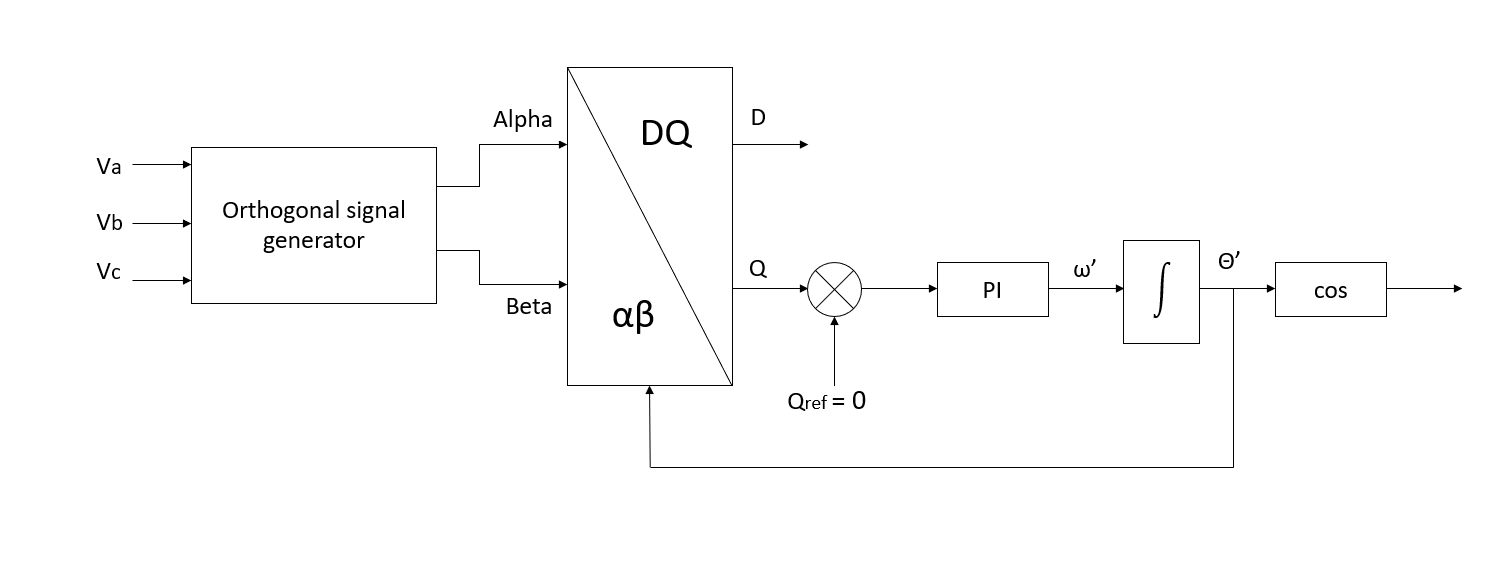
\includegraphics[width=1.0\textwidth]{SRF PLL.png}
      \caption{SRF-PLL Block diagram}
       \label{SRF-PLL}
\end{figure}

SRF-PLL with a high bandwidth can give a rapid and consistent detection of the phase and amplitude of the utility voltage vector under ideal utility conditions without any harmonic distortions or unbalance. If the utility voltage is distorted with high-order harmonics, the SRF-PLL can still operate if its bandwidth is decreased at the expense of PLL reaction time to reject and cancel the effect of these harmonics on the output \cite{guo2011phase}.
The three-phase SRF-PLL does not require three input signals to operate, as shown by the representation of the SRF-PLL in the stationary frame. It can work if it is given a phase-a signal and its orthogonal equivalent, which is a 90$^{\circ}$ phase shifted version of that signal \cite{silva2004performance}.
SRF-PLL provides average information rather than individual-phase frequency, amplitude, and phase measurements. 


\subsubsection{ Synchronous rotating reference frame}

In the SRF, the phase angle is tracked by synchronising the voltage space vector along the q or d axis \cite{ghoshal2007method}. The voltage space vector is synchronised with the q-axis in this example (figure 5.3).
%https://www.microsemi.com/document-portal/doc_view/132799-park-inverse-park-and-clarke-inverse-clarke-transformations-mss-software-implementation-user-guide

\begin{figure} 
    \centering
    \notag
    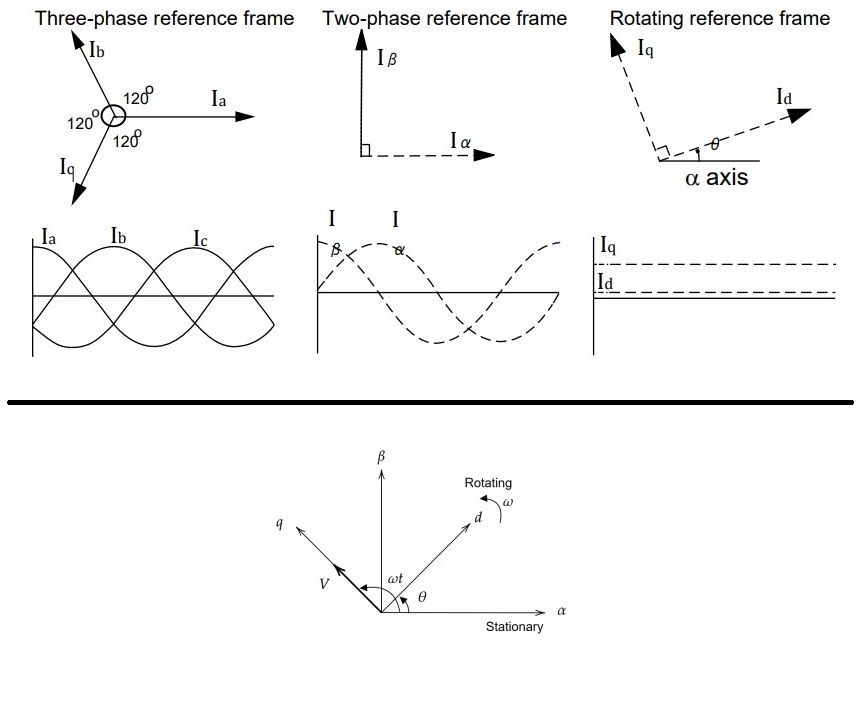
\includegraphics[width=0.8\textwidth]{reference frames_.jpg}
    \caption{Reference frames along with signal}
    \label{Reference frames along with signal}
\end{figure}

 This transformation synchronises the rotation of the two stationary axes with a reference frequency. The phase input $\omega$t is used to pass the reference frequency. There are two modes for rotating frame alignment:
\begin{enumerate}
    \item $0$ - The axis is aligned with the rotating frame. The outputs of this mode are $d = 0$ and $q = -1$ when the signals come from a balanced three-phase signal with unitary positive-sequence magnitude.
    \item $-pi/2$ - The rotating frame is $90^{\circ}$ behind the axis. The outputs of this mode are $d = 1$ and $q = 0$ when the signals come from a balanced three-phase signal with unitary positive-sequence magnitude.

\end{enumerate}

Alpha-beta to dq 0 alignment transformation matrix:

\begin{gather}
 \begin{bmatrix} d \\ q  \end{bmatrix}
 =
 \begin{bmatrix} \cos(\omega t) & \sin(\omega t) \\ -\sin(\omega t) & \cos(\omega t)  \end{bmatrix}
 \begin{bmatrix} \alpha \\ \beta  \end{bmatrix}
\end{gather}
\quad
Alpha-beta to dq -pi/2 alignment transformation matrix:

\begin{gather}
 \begin{bmatrix} d \\ q  \end{bmatrix}
 =
 \begin{bmatrix} \sin(\omega t) & -\cos(\omega t) \\ \cos(\omega t) & \sin(\omega t)  \end{bmatrix}
 \begin{bmatrix} \alpha \\ \beta  \end{bmatrix}
\end{gather}
\quad
In the current model the $-\pi /2$ behind the phase A alignment has been used.



In figure 5.3, different reference frames are represented along with the type of signal. When the values are DC (i.e., constant), different feedback controllers, such as proportional-integral (PI) and proportional-integral-derivative (PID), provide a pragmatic and reliable control solution. The Park transformation is used to convert two-axis orthogonal stationary reference frame quantities into rotating reference frame quantities. Below is given one simple example, which shows the same. 

\subsubsection{Park transformation or \textbf{$\alpha\beta$} to DQ transformation}

Suppose the input signal is, $V = V_g \sin{\omega t}$. 
Beta signal is taken as input, i.e., $V_{\beta} = V$. It's equivalent alpha signal is generated using a orthogonal signal generator. The alpha signal is $90^{\circ}$ phase shifted signal of the beta signal.

\begin{equation}
    V_{\beta} = V_g \sin{\omega t}     
\end{equation}
\begin{equation}
        V_{\alpha} = V_g \sin{(\omega t + \pi / 2)} \notag  
    \end{equation}
\begin{equation}    
        V_{\alpha} = V_g \cos{\omega t}
\end{equation}

Using the transformation matrix shown in equation 5.2, rotating reference frame quantities can be determined.

\begin{gather}
 \begin{bmatrix} V_d \\ V_q  \end{bmatrix}
 =
 \begin{bmatrix} \sin(\omega t) & -\cos(\omega t) \\ \cos(\omega t) & \sin(\omega t)  \end{bmatrix}
 \begin{bmatrix} V_{\alpha} \\ V_{\beta}  \end{bmatrix}
\end{gather}
\quad

from this, $V_d$ and $V_q$ can be determined for the reference frame.

\begin{gather}
 \begin{bmatrix} V_d \\ V_q  \end{bmatrix}
 =
 \begin{bmatrix} \sin(\omega t) & -\cos(\omega t) \\ \cos(\omega t) & \sin(\omega t)  \end{bmatrix}
 \begin{bmatrix} V_g \cos{\omega t} \\ V_g \sin{\omega t}  \end{bmatrix}
\end{gather}


\begin{gather}
 \begin{bmatrix} V_d \\ V_q  \end{bmatrix}
 =
 \begin{bmatrix} V_g \cos(\omega t) \sin(\omega t) - V_g \sin(\omega t) \cos(\omega t) \\ V_g \cos(\omega t) \cos(\omega t) + V_g \sin(\omega t) \sin(\omega t)  \end{bmatrix}
\end{gather}


\begin{gather}
 \begin{bmatrix} V_d \\ V_q  \end{bmatrix}
 =
 \begin{bmatrix} V_g \cos(\omega t) \sin(\omega t) - V_g \sin(\omega t) \cos(\omega t) \\ V_g \cos^{2}(\omega t)  + V_g \sin^{2}(\omega t)   \end{bmatrix}
\end{gather}


\begin{gather}
 \begin{bmatrix} V_d \\ V_q  \end{bmatrix}
 =
 \begin{bmatrix} 0 \\ V_g (\cos^{2}(\omega t)  + \sin^{2}(\omega t))   \end{bmatrix}
\end{gather}

\begin{gather}
 \begin{bmatrix} V_d \\ V_q  \end{bmatrix}
 =
 \begin{bmatrix} 0 \\ V_g    \end{bmatrix}
\end{gather}


It is seen in the equation 5.10, that $V_d = 0$ and $V_q = V_g$, which are constant values. 



\subsection{Generation of Alpha and Beta signals}

As seen in figure 5.4, the alpha and beta (Input) signals are generated using two low pass filters. Using one low pass filter will give us an equivalent signal with a 45 $^\circ$ phase shift. With two low pass filters using successively, a signal equivalent to input signal with 90$^\circ$ phase shift can be generated. The mathematics behind this, is shown below.

\begin{figure}[hbt!]
    \centering
    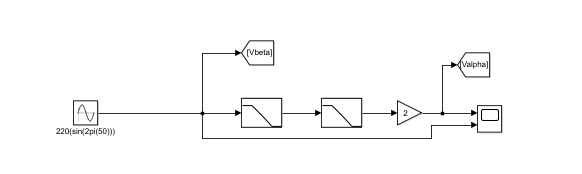
\includegraphics[width=1.0\textwidth]{GenAlphaBeta.png}
    \caption{Simulink model for generating Alpha Beta signals}
\end{figure}


\subsubsection{Mathematical logic }

The transfer function of a first order low-pass filter is given as,
\begin{equation}
  TF = \frac{\omega_c}{s + \omega_c}
  \end{equation}
Where, $\omega_c$ is the corner frequency of the low-pass filter.
Substituting, $s = j\omega$  in equation no (5.5),

\begin{equation}
  TF = \frac{\omega_c}{j\omega + \omega_c}
  \end{equation}
  
  From equation (5.6), The magnitude and phase of low-pass filter can be given as,
  
  \begin{equation}
      TF = \frac{\omega_c}{\sqrt{\omega^2 + \omega_c^2}} \quad \quad \phase{-\tan^{-1}{\frac{\omega}{\omega_c}}}
  \end{equation}

At cutoff frequency, i.e., $\omega = \omega_c$


 \begin{equation}
      TF = \frac{\omega}{\sqrt{\omega^2 + \omega^2}} \quad \quad \phase{ - \tan^{-1}{\frac{\omega}{\omega}}}
  \end{equation}

\begin{equation}
      TF = \frac{\omega}{\sqrt{\omega^2(2)}} \quad \quad \phase{ - \tan^{-1}{1}}
  \end{equation}
  
  \begin{equation}
      TF = \frac{\omega}{\omega \sqrt{2}} \quad \quad \phase{ - \frac{\pi}{4}}
  \end{equation}

\begin{equation}
      TF = \frac{1}{\sqrt{2}} \quad \quad \phase{ - 45^{\circ}}
  \end{equation}

When one more low-pass filter is used successively, the final magnitude and phase will become,

\begin{equation}
      TF = \frac{1}{\sqrt{2}} * \frac{1}{\sqrt{2}} \quad \quad \phase{ - 45^{\circ} + (-45^{\circ})}
  \end{equation}

\begin{equation}
      TF = \frac{1}{2} \quad \quad \phase{- 90^{\circ}}
  \end{equation}

As seen here, the magnitude of final signal is becoming half of what it was before. To compensate for this, gain of 2 has been used at the end as shown in figure 5.4. The output at the end of the gain is the equivalent of the input signal with 90$^{\circ}$ phase shift. Upon running the simulation, the generated alpha and beta signals are shown in figure 5.5.   

\begin{figure}[hbt!]
    \centering
    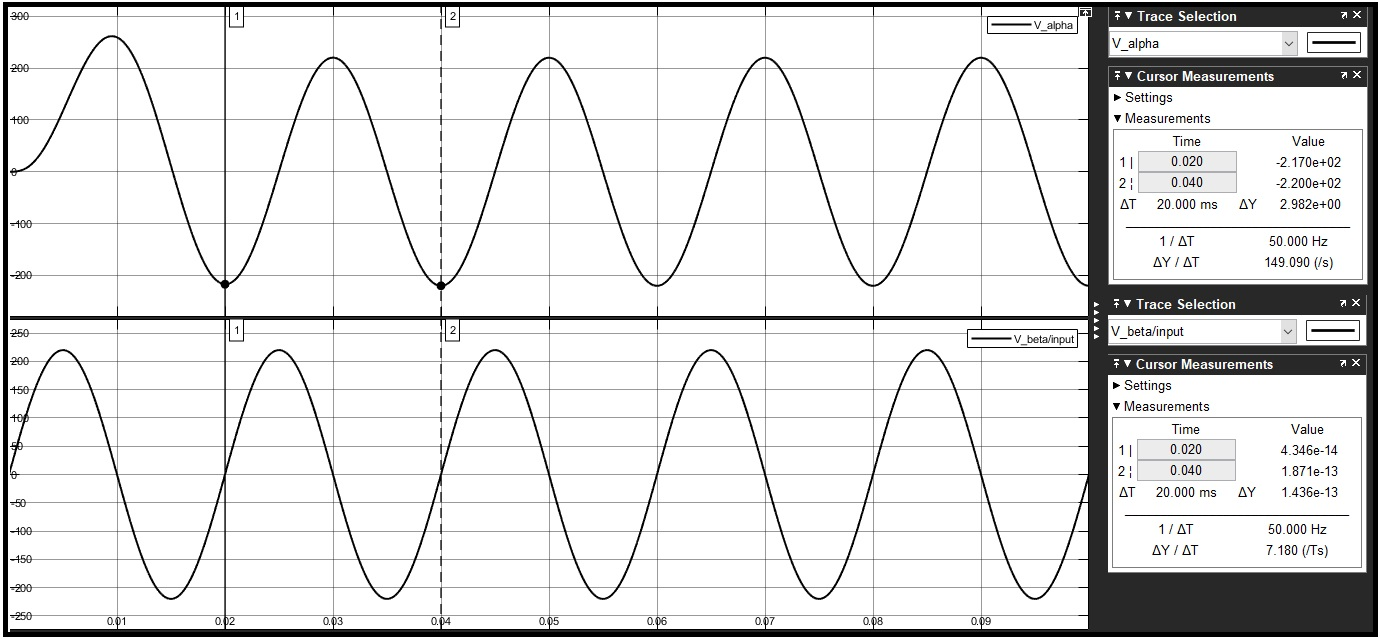
\includegraphics[width=1.0\textwidth]{AlphaBeta_one signal.jpg}
    \caption{Alpha beta signals}
\end{figure}






\section{The MATLAB Simulink model and simulations for SRF-PLL}

The three phase SRF-PLL model can be used to make single phase SRF-PLL, not in a straightforward manner but it provides a useful structure for single-phase PLLs as long as the 90-degree-shifted orthogonal component of the single-phase input signal is created \cite{silva2004performance}.  The model is Shown in fig 5.6. The solver configurations and all of the important block parameters to run the simulation are shown in Appendix B. 

\begin{figure}[hbt!]
    \centering
    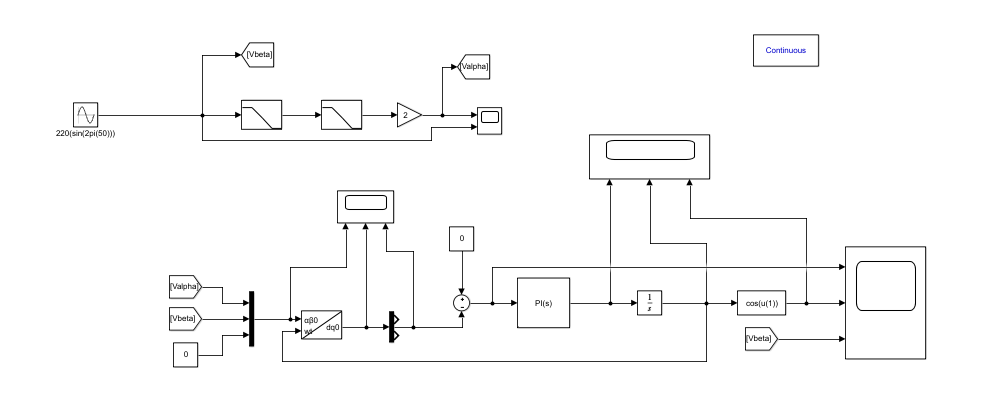
\includegraphics[width=1.0\textwidth]{Screenshot 2021-05-29 005435.png}
    \caption{SRF-PLL MATLAB Simulink model}
\end{figure}



\subsection{Simulation with a constant sinusoidal input signal (Input signal without disturbances)}

The ideal case is when the input signal to the SRF-PLL has no disturbances , i.e., it's frequency, amplitude and Phase remains same always, that too without any harmonics. The model shown in figure 5.6 is constructed for such a case in simulink. 
The input signal given is $220\sin{2 \pi 50}$, which is also the beta signal for the model. The simulation is run for 0.1 seconds, with variable type step solver (Ode 45, Dormand-prince) with min step being $10^{-8}$ and maximum step being $10^{-7}$. The output signal is shown in figure 5.7. For an ideal signal, the PLL is giving the desired output. As seen in the error signal, in figure 5.7, it takes approximately $2.1 mS$ for the system to become steady. 


 \begin{figure}[hbt!]
    \centering
    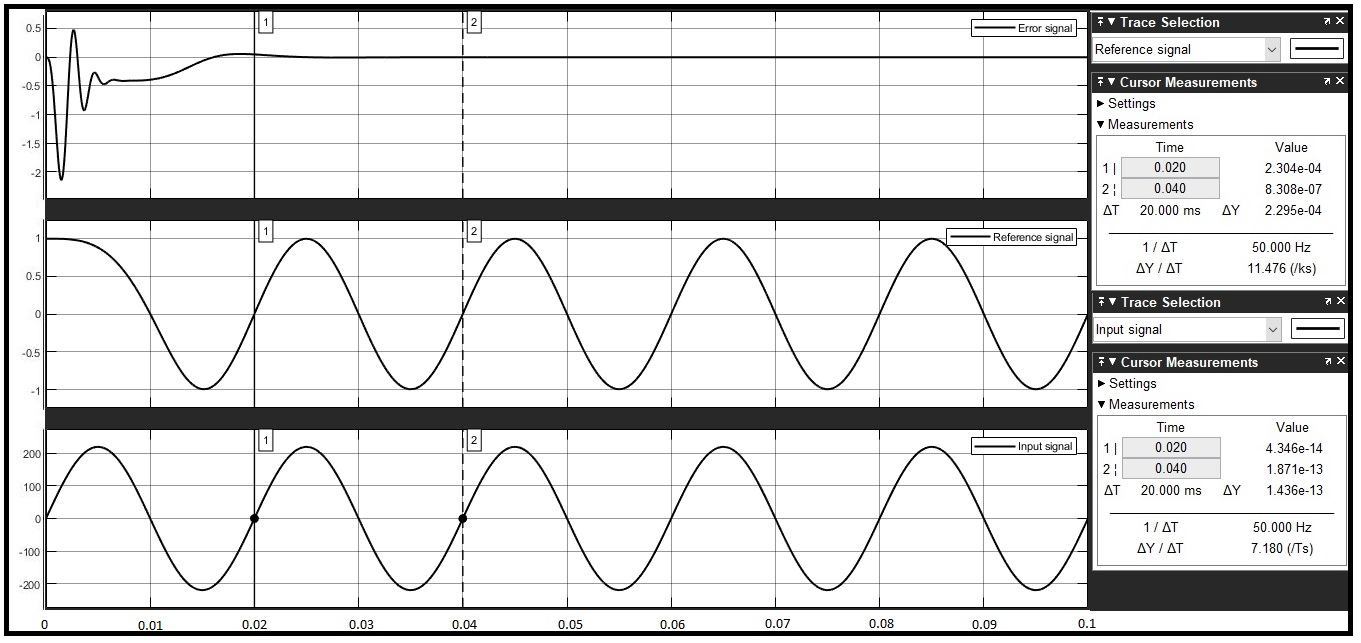
\includegraphics[width=1.0\textwidth]{output_one signal.jpg}
    \caption{Constant Sinusoidal signal ($220\sin{2 \pi 50}$), ideal case output}
\end{figure}

\subsection{Simulation with step variation of Frequency, Phase and Amplitude (Input signal with disturbances)}

A PLL should be able to synchronise the grid's voltage and the inverter's current using a reference signal, even if there are disturbances in the grid. To realise such a case where there are frequency, phase and amplitude disturbances, the Simulink model shown in figure 5.8 is used. the input signal is varied using a MATLAB function block of Simulink with a simple code, shown in appendix A, which will pass one signal for a period of time then pass the other signal for a the next time period.

\subsubsection{Step variation of frequency}

As shown in Fig 5.8, when the clock is 1, the Matlab function block will pass the signal with $51hz$  frequency, $220\sin{2\pi51}$, for first half of the simulation time period, and then it will pass the signal with $50hz$ frequency, $220\sin{2\pi50}$. The input signal can be seen in figure 5.9. The alpha beta signals that are generated is shown in figures 5.10 and figure 5.11. The reference signal generated along with the error signal is shown in figure 5.12. The output at the end is what is desired, i.e, the PLL is tracking the input signal when the frequency varies.

\begin{figure}[hbt!]
    \centering
    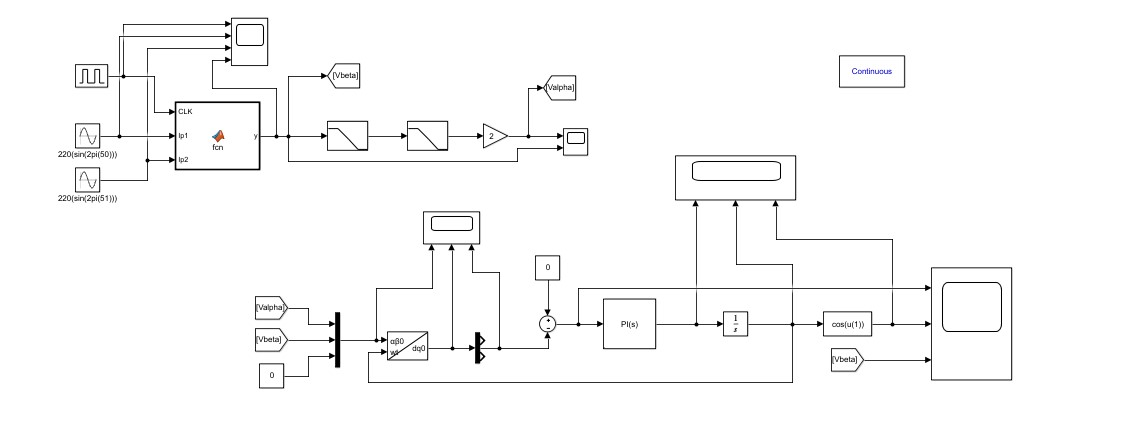
\includegraphics[width=1.0\textwidth]{Model simulation.jpg}
    \caption{Simulink model for Step variation of frequency}
\end{figure}

\begin{figure}[hbt!]
    \centering
    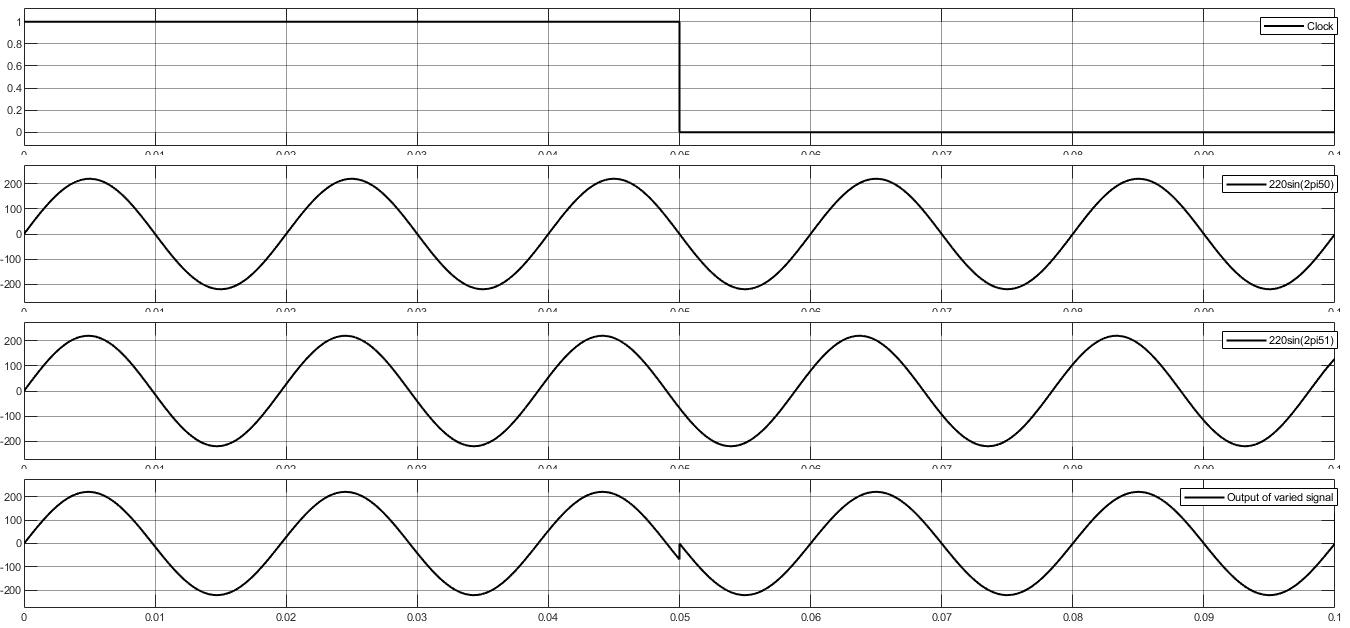
\includegraphics[width=1.0\textwidth]{Step variation of frequency.jpg}
    \caption{Input for step variation of frequency}
\end{figure}

\begin{figure}[hbt!]
    \centering
    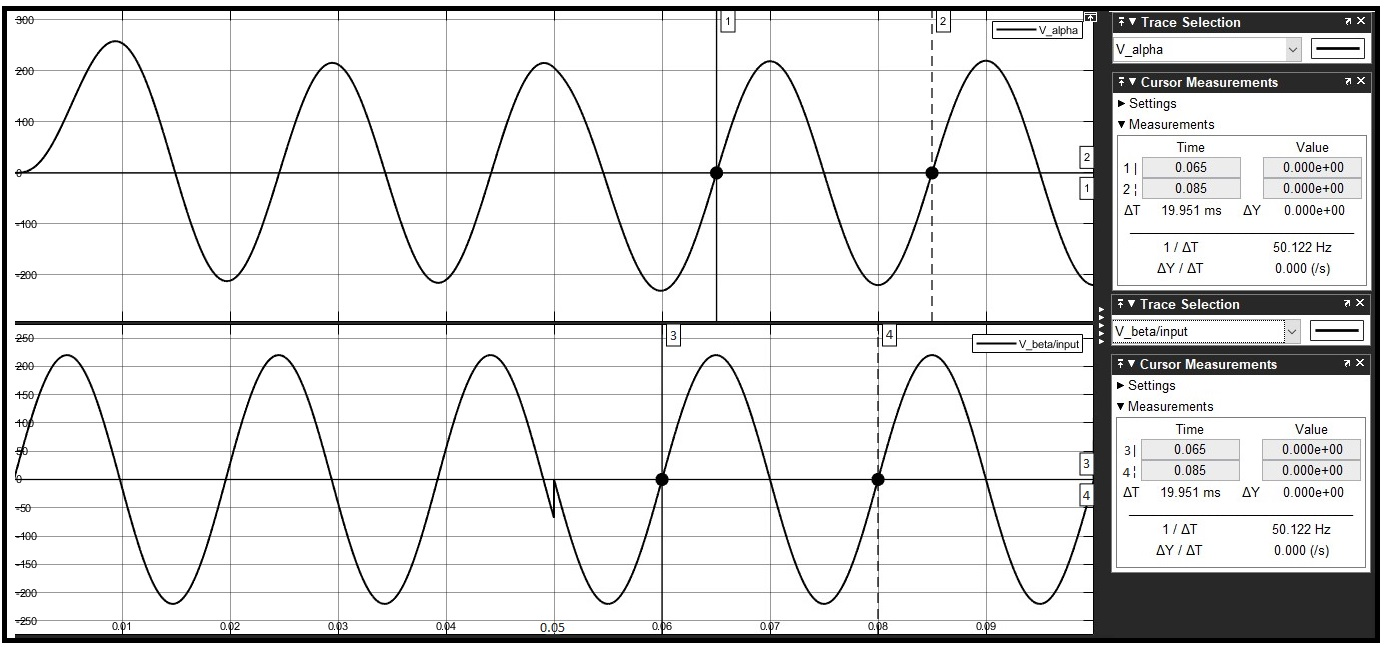
\includegraphics[width=1.0\textwidth]{alhpa_beta (50hz).jpg}
    \caption{Alpha beta signals generated for variation of frequency (50hz)}
\end{figure}

\begin{figure}[hbt!]
    \centering
    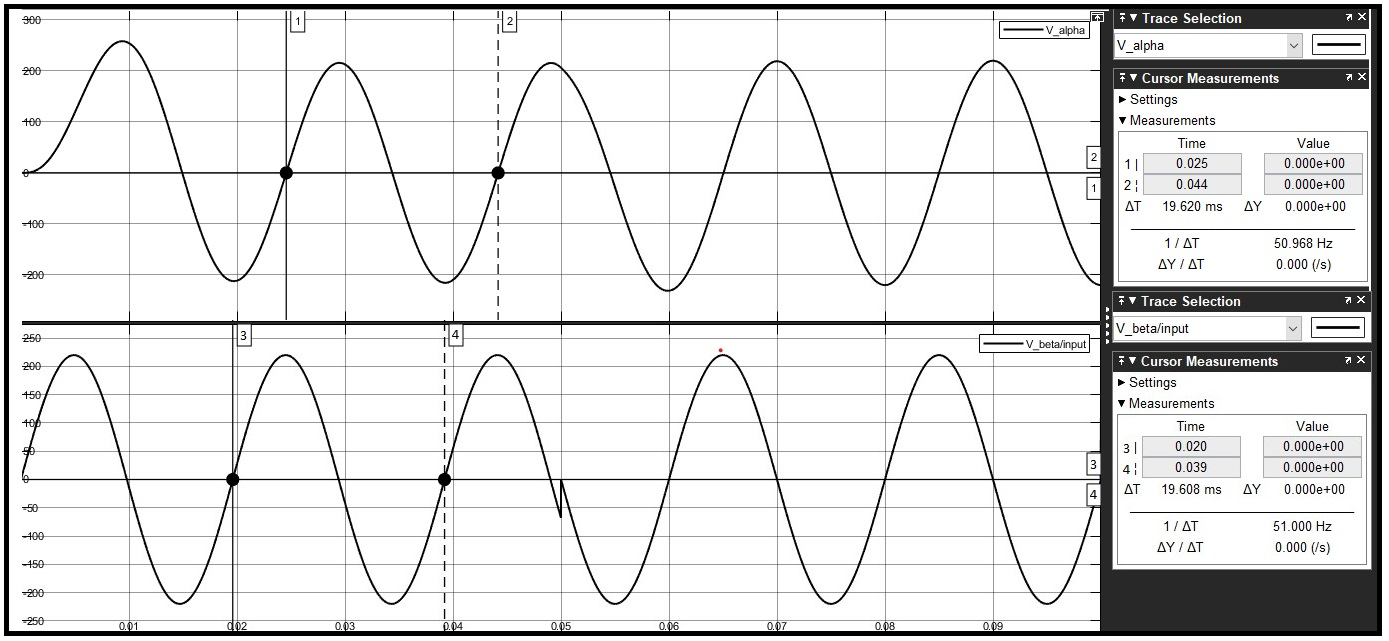
\includegraphics[width=1.0\textwidth]{alhpa_beta (51hz).jpg}
    \caption{Alpha beta signals generated for variation of frequency (51hz)}
\end{figure}


\begin{figure}[hbt!]
    \centering
    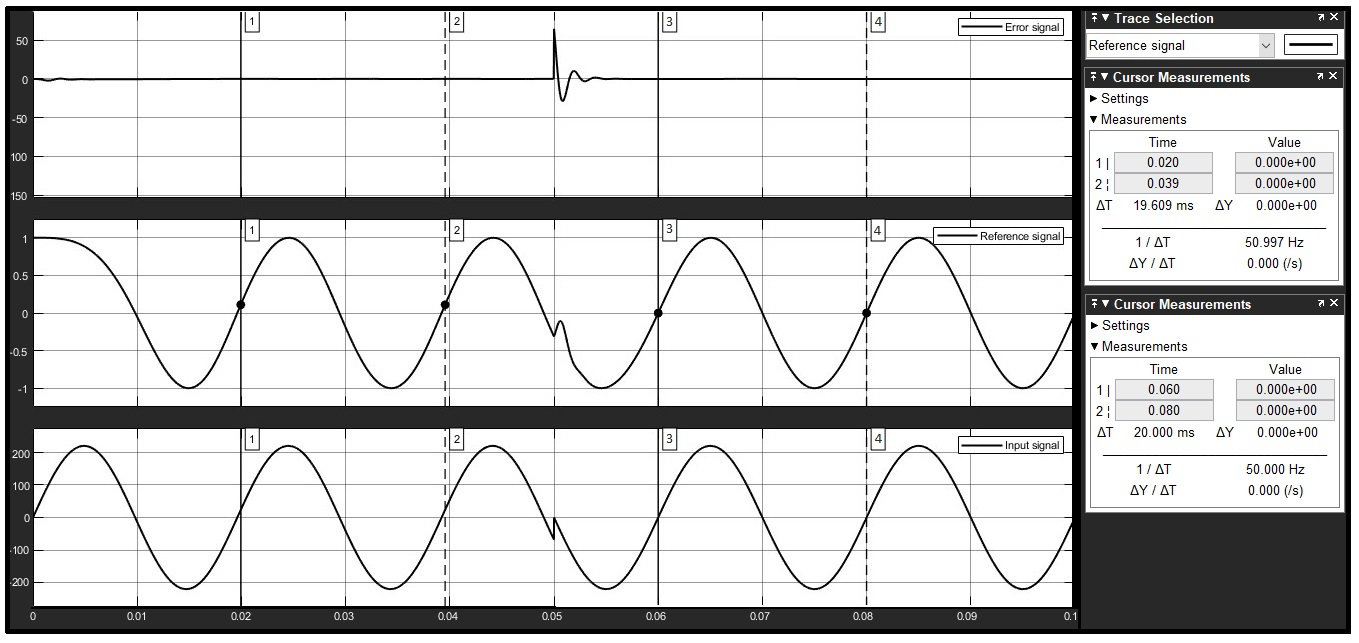
\includegraphics[width=1.0\textwidth]{Output.jpg}
    \caption{output with Step variation of frequency}
\end{figure}


\subsubsection{Step variation of Phase}

The same Matlab function block is used again with different input signals. The simulink model can be seen in figure. 5.13.
Both having the same frequency and amplitude but with different phase. There's 10$^{\circ}$ of phase difference between these two input signals. The input signal can be seen in figure 5.14. The generated alpha beta signals are shown in figure 5.15. The output reference signal along with error signal is shown in figure 5.16. It is seen in figure 5.16 that PLL is able to track the input signal as the output signal has same phase as the input signal phase.
\begin{figure}[hbt!]
    \centering
    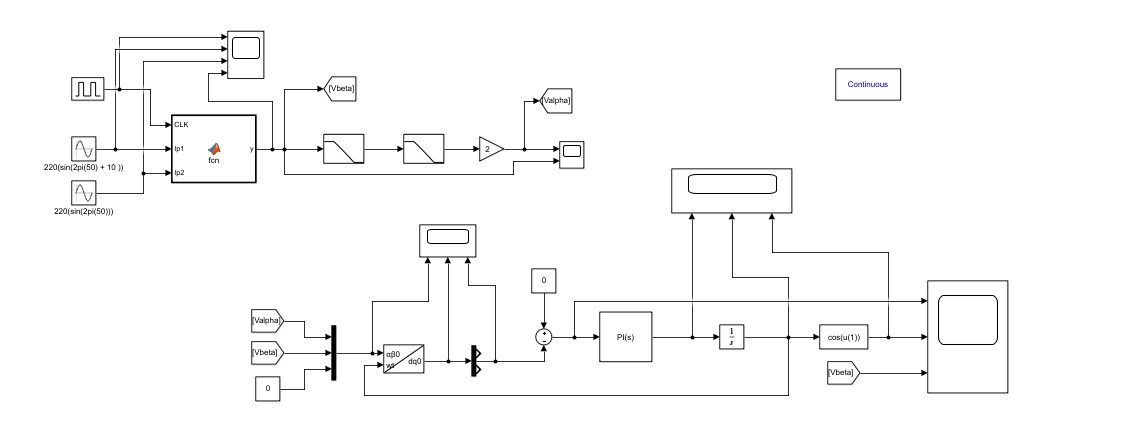
\includegraphics[width=1.0\textwidth]{Step variation of phase.jpg}
    \caption{Simulink model for Step variation of Phase}
\end{figure}



\begin{figure}[hbt!]
    \centering
    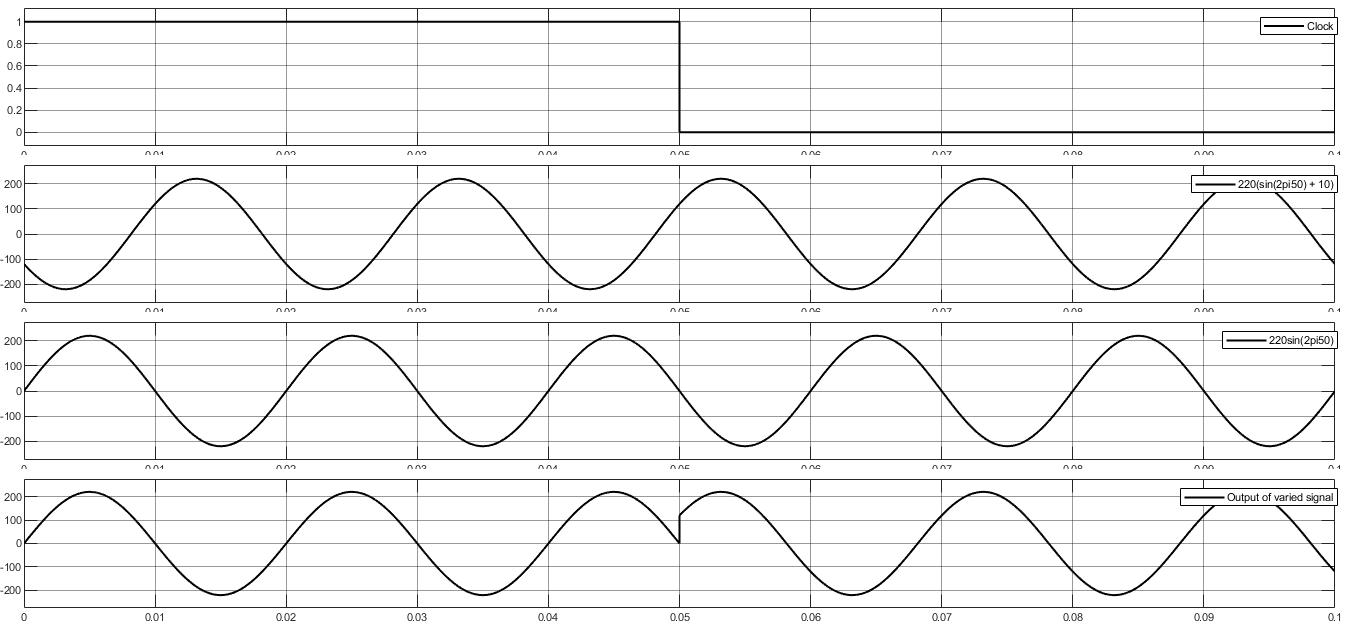
\includegraphics[width=1.0\textwidth]{input_phase.jpg}
    \caption{Input for Step variation of Phase}
\end{figure}



\begin{figure}[hbt!]
    \centering
    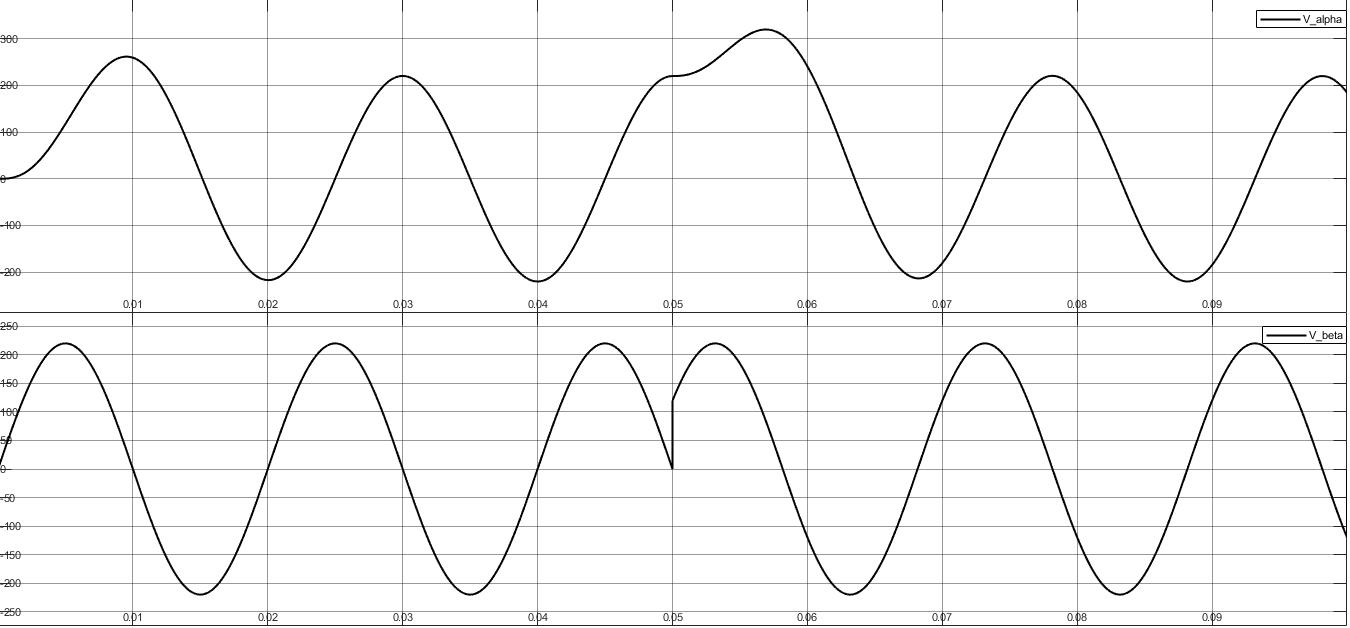
\includegraphics[width=1.0\textwidth]{alphaBeta_Phase.jpg}
    \caption{Alpha beta signals generated for variation of Phase}
\end{figure}


\begin{figure}[hbt!]
    \centering
    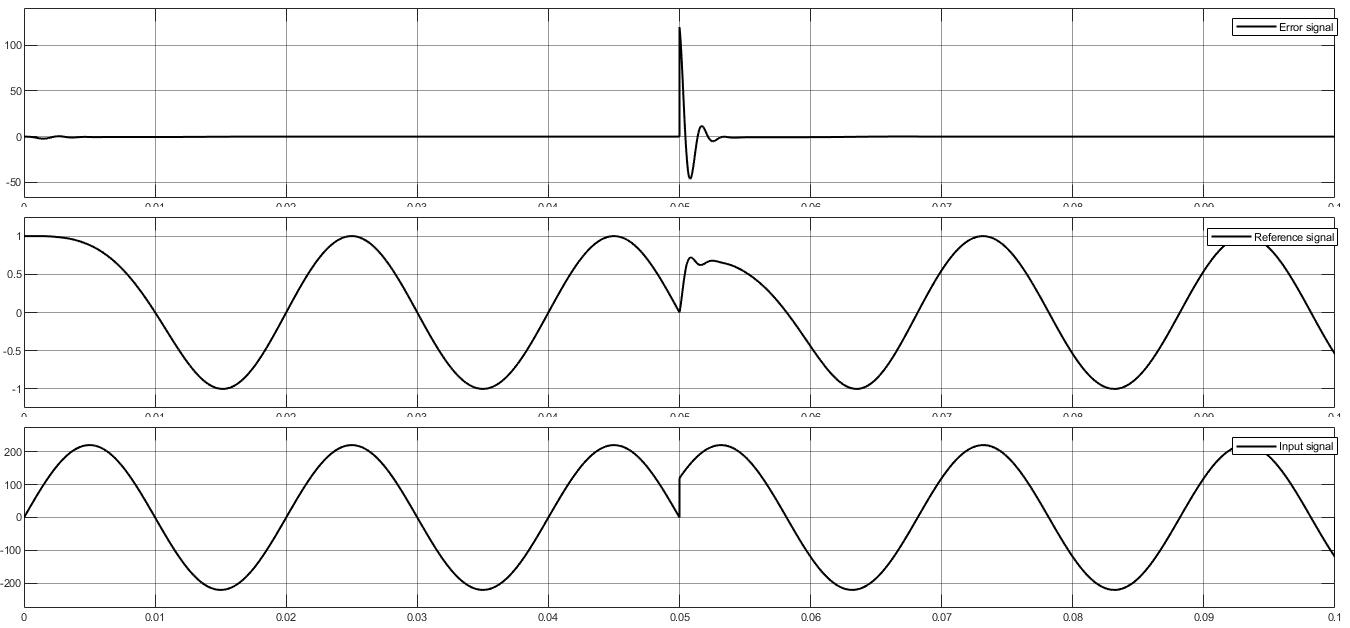
\includegraphics[width=1.0\textwidth]{output_phase.jpg}
    \caption{output with Step variation of Phase}
\end{figure}

\subsubsection{Step variation of Amplitude}

Different input signals are used with the same Matlab Function block. The simulink model can be seen in figure. 5.17.
Both having the same frequency and Phase but with different Amplitude. One signal has $230$ amplitude and the other one has $220$.The difference in amplitude can be seen by a horizontal line stretched using measurement feature of Scope block shown in figure 5.18. The input signal can be seen in figure 5.18. The generated alpha beta signals are shown in figure 5.19. The output reference signal along with error signal is shown in figure 5.20., in which it is seen that amplitude variation in input signal has no effect on the reference signal generated.
\begin{figure}[hbt!]
    \centering
    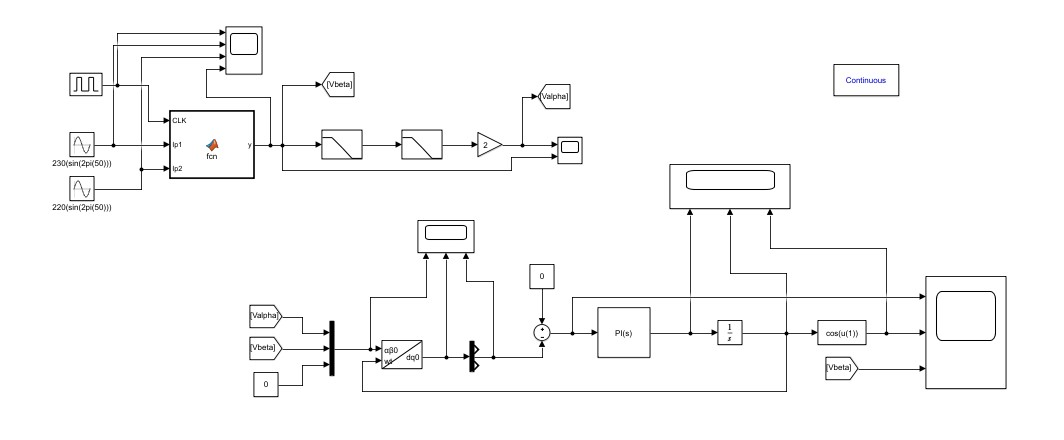
\includegraphics[width=1.0\textwidth]{Step variation of amplitude.jpg}
    \caption{Simulink model for Step variation of amplitude}
\end{figure}



\begin{figure}[hbt!]
    \centering
    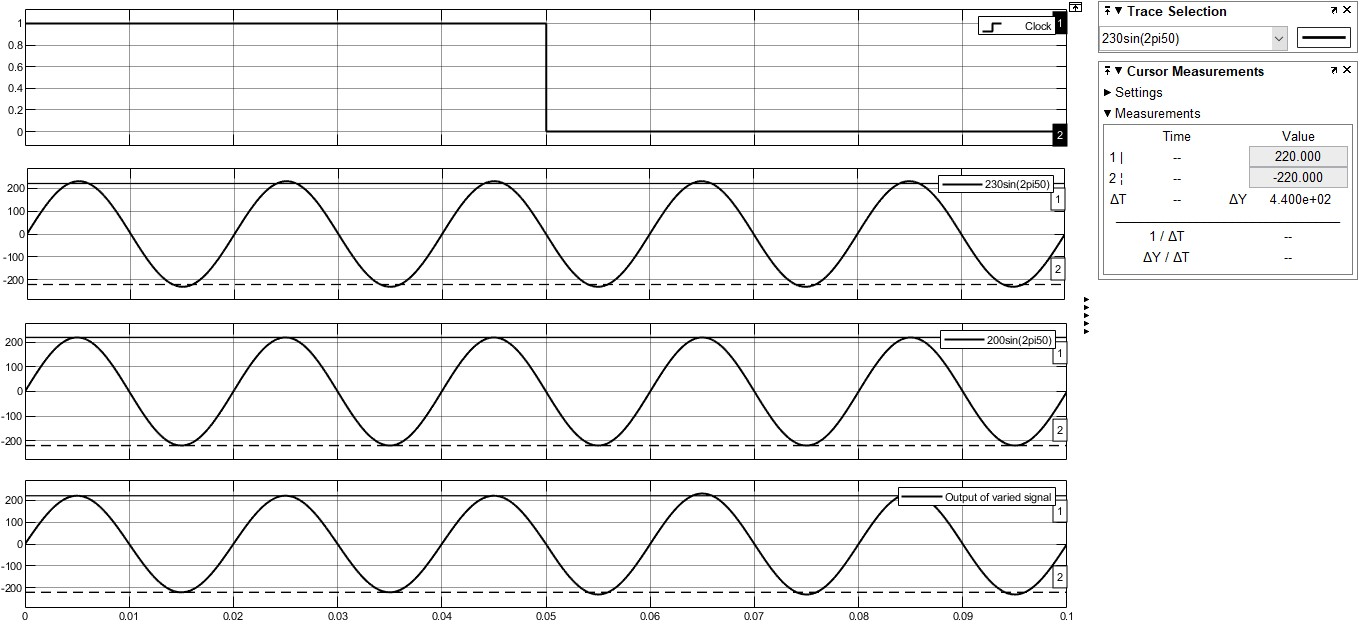
\includegraphics[width=1.0\textwidth]{amp_input.jpg}
    \caption{Input for Step variation of Amplitude}
\end{figure}



\begin{figure}[hbt!]
    \centering
    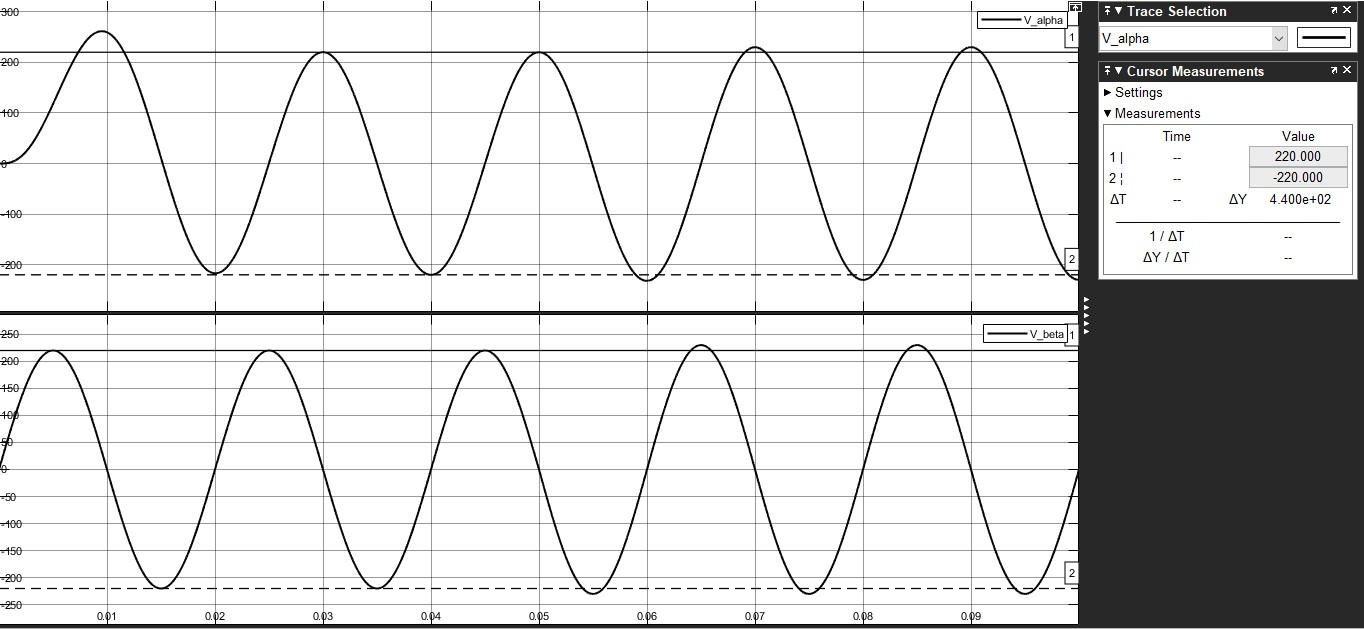
\includegraphics[width=1.0\textwidth]{amp_alphabeta.jpg}
    \caption{Alpha beta signals generated for variation of Amplitude}
\end{figure}


\begin{figure}[hbt!]
    \centering
    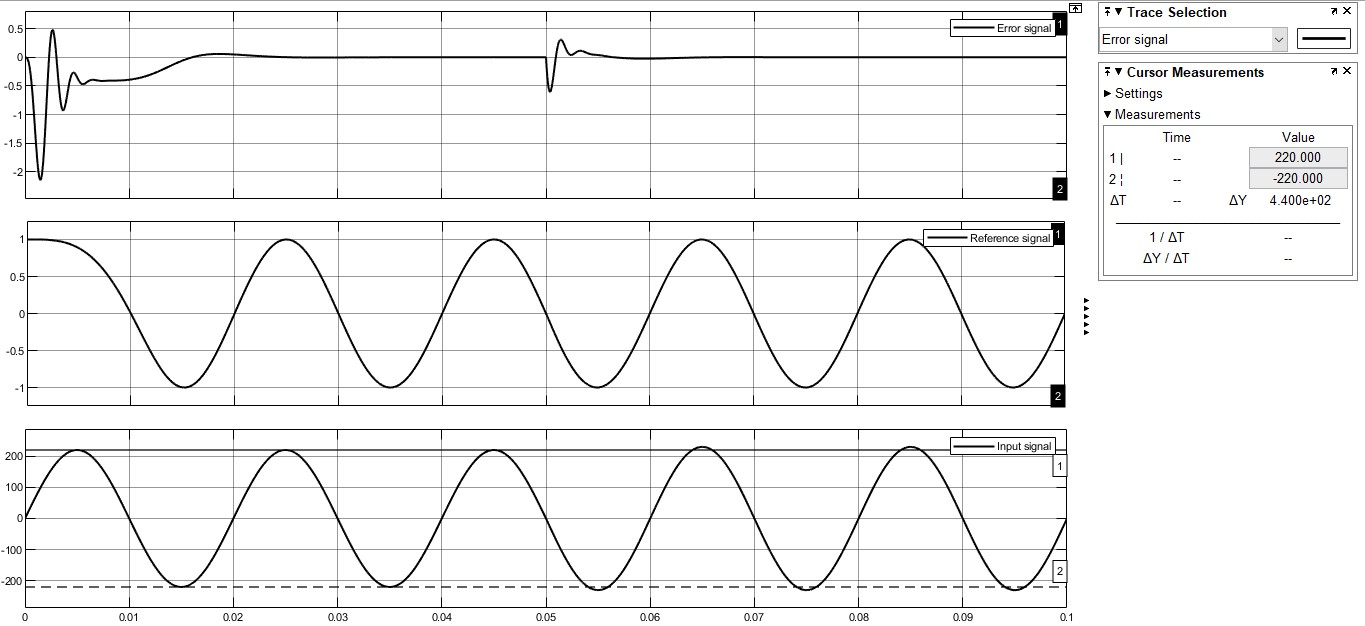
\includegraphics[width=1.0\textwidth]{amp_output.jpg}
    \caption{output with Step variation of Amplitude}
\end{figure}


\subsection{Simulation with Harmonics in the input signal}

The model is tested for the input signal with general harmonics found in the transmission/distribution network. The current amount of harmonic pollution in the Indian power system is investigated in this research \cite{jain2004survey}. Also investigated is the harmonic content of some of the most widely utilised loads and residential regions. In addition, a survey is given in order to determine the harmonic level existing in the distribution system. It has been noted that the voltages on transmission/distribution systems have substantially less distortion, according to the analysis on the distribution network. However, as we get closer to the load, the voltage distortion rises. At the customer's end, significant distortion is recorded, with a high percentage of $5^{th}$ and $7^{th}$ harmonic components. From this study, to observe the injection of harmonics on the system a signal with $5^{th}$ and $7^{th}$ harmonic components is given to the SRF-PLL. 
The Simulink model for this test is shown in figure 5.21. The input signal with harmonic components in it are shown in figure 5.22. It's result is shown in figure 5.53. As seen from the results, the SRF-PLL model shown in the project is not able to track the fundamental component of the input signal.


\begin{figure}[hbt!]
    \centering
    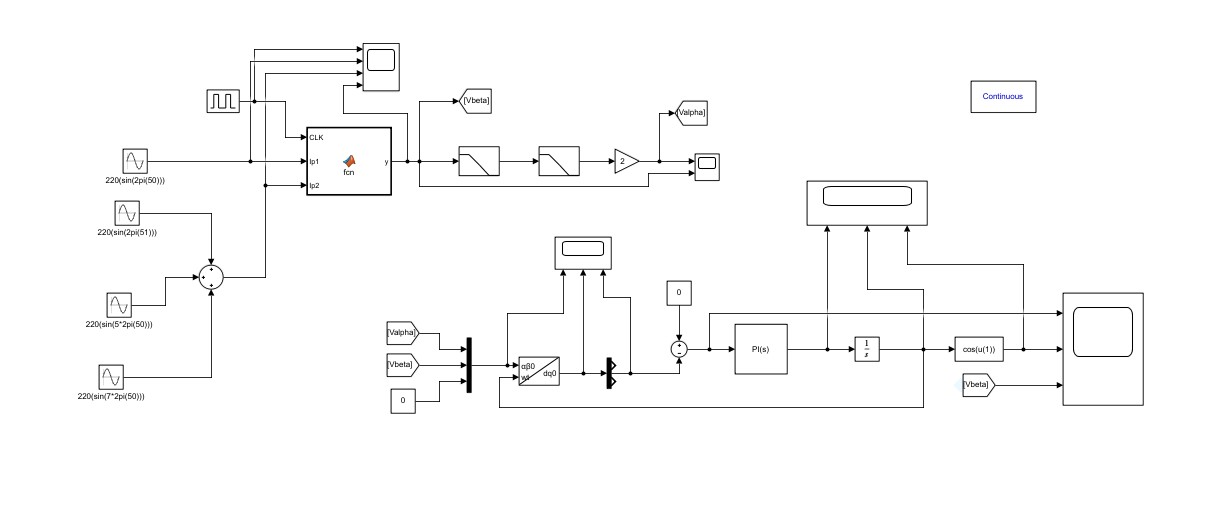
\includegraphics[width=1.0\textwidth]{Harmonics_model.jpg}
    \caption{Simulink model for a signal with Harmonics}
\end{figure}

\begin{figure}[hbt!]
    \centering
    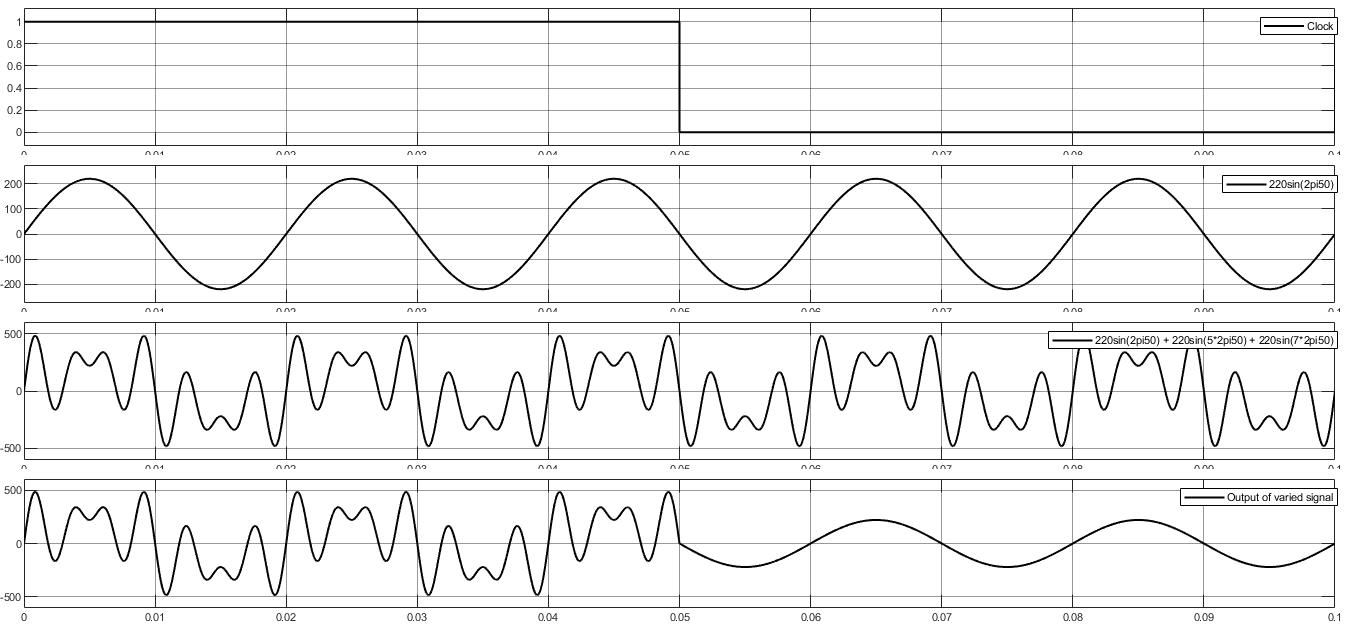
\includegraphics[width=1.0\textwidth]{Harmonics_Input.jpg}
    \caption{Input signal: Harmonics injected signal}
\end{figure}

\begin{figure}[hbt!]
    \centering
    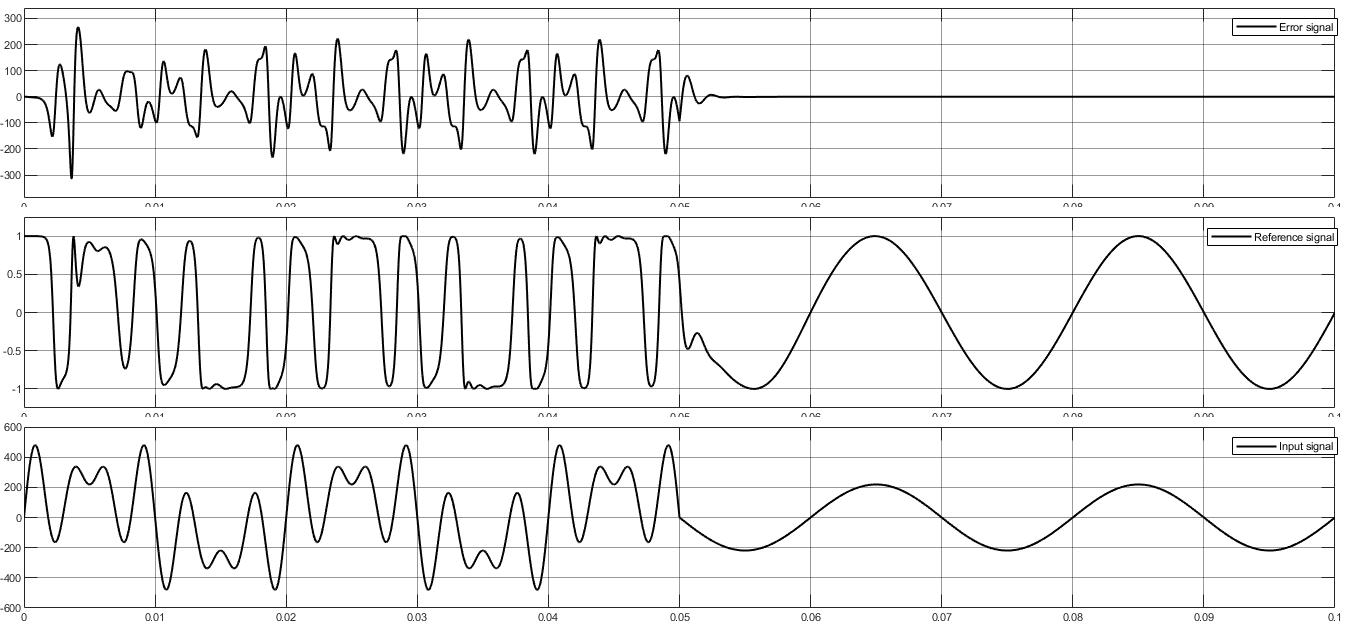
\includegraphics[width=1.0\textwidth]{Harmonics_Outpu.jpg}
    \caption{Output for the signal with Harmonics}
\end{figure}




\section{Code generation for STM32F4 discovery board}
Codes compatible with STM32F4 discovery board micro-controller are generated using Embedded coder application of MATLAB. The configuration files used to select the pins of micro-controller are made using STMicroelectronics application named, STM32CubeMX. The target file used to generate the code is stm32.tlc, which is seen in the appendix B where the block parameters and configurations are given.
The generated code for model and it's header files along with other helpful header files are given in Appendix B.

\chapter{Conclusion}

The model of inverter system was prepared with MPPT and the control strategy was devised for the same. Its implementation on STM discovery board was tried. On changing irradiance and temperature values the MPPT corresponded to the change in condition and thus it tracked the new MPP.
\\The SRF-PLL model shown here is highly accurate and has response time of approximately $4.5mS$. The simulations revealed that for ideal signal, as seen in the figure 5.7, the error signal is being stable after $0.02S$. When there is a step variation in frequency, phase and amplitude the model has accurate results but a signal with harmonics it can not track.
%%%%%%%%%%%%%%%%%%%%%%%%%%%%%%%%%%%%%%%%%%%%%%%%%%%%%%%%%%%%
% Appendices.

\begin{appendices}

\appendix

\chapter{Waijung Models}
\label{Models created using Waijung Library}
These are basic models created using waijung library for a proper understanding of its simulink blocks.

\begin{figure}[hbt!]
    \centering
    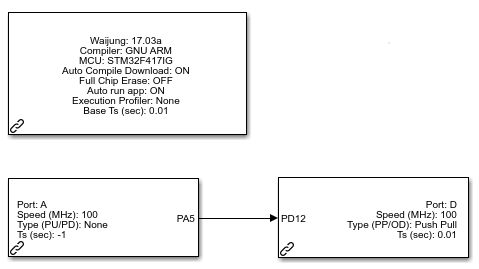
\includegraphics{digital input.png}
    \caption{Model for turning on LED by giving input to pin PA5}
\end{figure}

\begin{figure}[hbt!]
    \centering
    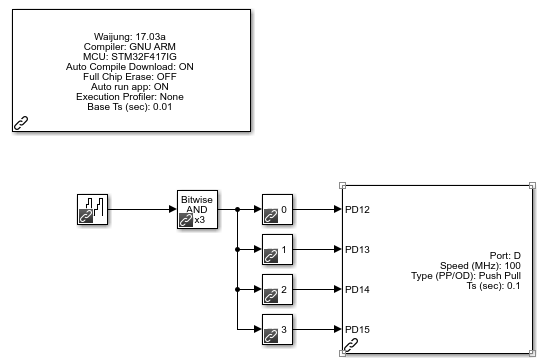
\includegraphics{digital output.png}
    \caption{Model for turning on/off led repeatedly.}
\end{figure}

\newpage
\begin{figure}[hbt!]
    \centering
    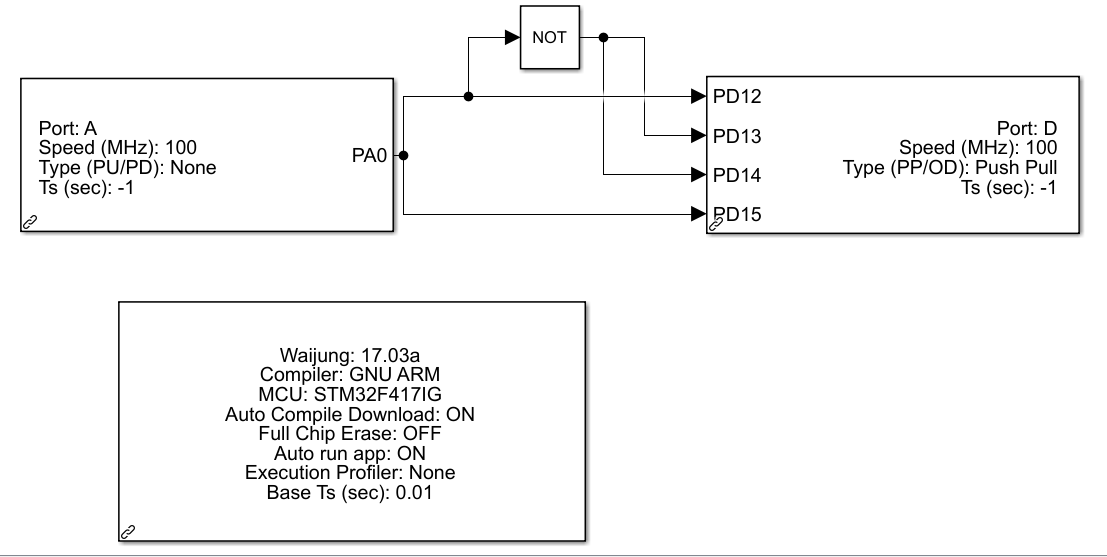
\includegraphics[width=14cm,height=9cm]{turiningonoffswitch.png}
    \caption{Model for switching on/off led by pressing switch.}
\end{figure}


\chapter{STM codes}
\label{STM Demo Codes}
These following codes are written in Atollic true studio for STM32. These are demo codes written for proper understanding of its library functions.

\section{Code for controlling switching of on/off for path P1 and P2}
\begin{lstlisting}[language=C++]

#include "stm32f4xx.h"                           /* Include STM Inbuilt Library*/
#include "stm32f4_discovery.h"

GPIO_InitTypeDef GPIO_C1;                        /* Initaializing the function */

int main(void)                                  /* Starting The main function */
{

  RCC_AHB1PeriphClockCmd(RCC_AHB1Periph_GPIOA, ENABLE);        /* Initializing the clock for portA and enabling it */
  RCC_AHB1PeriphClockCmd(RCC_AHB1Periph_GPIOD, ENABLE);        /* Initializing the clock for portD and enabling it */
  RCC_AHB1PeriphClockCmd(RCC_AHB1Periph_GPIOE, ENABLE);       /* Initializing the clock for portE and enabling it */

  GPIO_C1.GPIO_Pin = GPIO_Pin_5;                         /* Initializing the Pin PA5 */
  GPIO_C1.GPIO_OType = GPIO_OType_PP;                    /* Initializing the Pin to work in push pull mode */
  GPIO_C1.GPIO_Mode = GPIO_Mode_IN;                      /* Initializing the Pin PA5 to work in Input Mode */
  GPIO_C1.GPIO_PuPd = GPIO_PuPd_NOPULL;                  /* Initializing the Pin PA5 to work as No pull means no low or high */
  GPIO_C1.GPIO_Speed = GPIO_Speed_50MHz;                /* Initializing the spped of clock pulse */
  GPIO_Init(GPIOA, &GPIO_C1);                           /* Calling the function Init by passing two values*/


  GPIO_C1.GPIO_Pin = GPIO_Pin_12;                      /* Initializing the Pin PD12 */
  GPIO_C1.GPIO_Pin = GPIO_Pin_13;                      /* Initializing the Pin PD13 */
  GPIO_C1.GPIO_OType = GPIO_OType_PP;                  /* Initializing the Pin PD12, PD13 to work in Push Pull Mode */
  GPIO_C1.GPIO_Mode = GPIO_Mode_OUT;                  /* Initializing the Pin PD12, PD13 to work in output mode */
  GPIO_C1.GPIO_PuPd = GPIO_PuPd_NOPULL;               /* Initializing the Pin PD12, PD13 to work as no pull mode */
  GPIO_C1.GPIO_Speed = GPIO_Speed_50MHz;             /* Initializing the spped of clock pulse */
  GPIO_Init(GPIOD, &GPIO_C1);                        /* Calling the function Init by passing two values*/


  GPIO_C1.GPIO_Pin = GPIO_Pin_11;                     /* Initializing the Pin PE11 */
  GPIO_C1.GPIO_Pin = GPIO_Pin_13;                      /* Initializing the Pin PE13 */
  GPIO_C1.GPIO_OType = GPIO_OType_PP;                   /* Initializing the Pin PE1, PE13 to work in push pull mode */
  GPIO_C1.GPIO_Mode = GPIO_Mode_OUT;                    /* Initializing the Pin PE11, PE13 to work in output mode */
  GPIO_C1.GPIO_PuPd = GPIO_PuPd_NOPULL;                  /* Initializing the Pin PE11, PE13 to work as no pull mode */
  GPIO_C1.GPIO_Speed = GPIO_Speed_50MHz;              /* Initializing the Speed of clock pulse */
  GPIO_Init(GPIOE, &GPIO_C1);                        /* Calling the function Init by passing two values*/

  while (1)
  {
	if(GPIO_ReadInputDataBit(GPIOA, GPIO_Pin_5) == Bit_SET)        /* Checking if Input is High or not */
	{
		GPIO_WriteBit(GPIOD, GPIO_Pin_12, Bit_SET);             /* Making pin PD12 set high */
		GPIO_WriteBit(GPIOE, GPIO_Pin_11, Bit_SET);             /* Making pin PE11 set high */
	}
	else
	{
		GPIO_WriteBit(GPIOD, GPIO_Pin_13, Bit_SET);             /* Making Pin PD13 set high */
		GPIO_WriteBit(GPIOE, GPIO_Pin_11, Bit_RESET);           /* Making Pin PE11 set low */
		GPIO_WriteBit(GPIOE, GPIO_Pin_13, Bit_SET);             /* Making Pin PE13 set high */
	}
  }
}


\end{lstlisting}

\section{Code for MPPT}
\begin{lstlisting}[language=C++]
#include "stm32f4xx.h"
#include "stm32f4_discovery.h"

GPIO_InitTypeDef  GPIO_RefGen;           /* Defining the function*/

int Vrefmax = 363;                       /* Assuming the Vref maximun value*/
int Vrefmin = 0;                         /* Assuming the Vref minimum value*/
int Vrefinit = 300;                      /* Assuming Vrefinit value as 300 coz at here MPP occurs*/
int deltaVref = 1;                       /* Taking a constant value*/

double Vold = 0;double Pold = 0;       /*declaring values and variables*/
double Vrefold = 300;double V;
double P;double I;
double dV;double dP;double Vref;

int main(void)                         /*Starting the main function*/
{
	RCC_AHB1PeriphClockCmd(RCC_AHB1Periph_GPIOA, ENABLE);    /*initializing the clock pulses*/
	RCC_AHB1PeriphClockCmd(RCC_AHB1Periph_GPIOD, ENABLE);
	
	GPIO_RefGen.GPIO_Pin = GPIO_Pin_5;                    /*Initializing the pin*/
	GPIO_RefGen.GPIO_OType = GPIO_OType_PP;
	GPIO_RefGen.GPIO_Mode = GPIO_Mode_IN;
	GPIO_RefGen.GPIO_Speed = GPIO_Speed_50MHz;
	GPIO_RefGen.GPIO_PuPd = GPIO_PuPd_NOPULL;
	GPIO_Init(GPIOA, &GPIO_RefGen);
	
	
	GPIO_RefGen.GPIO_Pin = GPIO_Pin_12;
	GPIO_RefGen.GPIO_OType = GPIO_OType_PP;
	GPIO_RefGen.GPIO_Mode = GPIO_Mode_IN;
	GPIO_RefGen.GPIO_Speed = GPIO_Speed_50MHz;
	GPIO_RefGen.GPIO_PuPd = GPIO_PuPd_NOPULL;
	GPIO_Init(GPIOD, &GPIO_RefGen);
    


  while (1)
  {
	V = GPIO_ReadInputData(GPIOA);
	I = GPIO_ReadInputData(GPIOD);
	P = V*I;
	dV = V - Vold;
	dP = P - Pold;
	
	if (dP == 0)
	{
		Vref = Vrefold;
	}
	
	if (dP < 0)
	{
		if (dV < 0)
		{
			Vref = Vrefold + deltaVref;
		}
		else
		{
			Vref = Vrefold - deltaVref;
		}
		
	}
	
	if (dP > 0)
	{
		if (dV < 0)
		{
			Vref = Vrefold - deltaVref;
		}
		else
		{
			Vref = Vrefold + deltaVref;
		}
	}
	if (Vref >= Vrefmax || Vref <= Vrefmin)
	{
		Vref = Vrefold;
	}
	Vrefold = Vref;
	Vold = V;
	Pold = P;
  }
}
\end{lstlisting}



\section{Code for Glowing LED for an infinite period.}
\begin{lstlisting}[language=C++]
#include "stm32f4xx.h"             /*Inculde STM inbuilt library*/
#include "stm32f4_discovery.h"

GPIO_InitTypeDef GPIO_LED;           /* Initializing the function */

int main(void)   /* Begining the main function */
{

  RCC_AHB1PeriphClockCmd(RCC_AHB1Periph_GPIOD, ENABLE);       /* Initializing and starting the clock of Port D */

  GPIO_LED.GPIO_Pin = GPIO_Pin_12;          /* Initializing the Pin 12 */
  GPIO_LED.GPIO_Mode = GPIO_Mode_OUT;       /* Initializing the Pin 12 in output mode */
  GPIO_LED.GPIO_OType = GPIO_OType_PP;      /* Initializing the Pin 12 with Push Pull mode */
  GPIO_LED.GPIO_Speed = GPIO_Speed_50MHz;   /* Initializing the port D with the clock speed */

  GPIO_Init(GPIOD, &GPIO_LED);             /* Calling the function Init by passing two values */

  GPIO_WriteBit(GPIOD, GPIO_Pin_12, Bit_SET);  /* Making pin PD12 set high by passing Bit_SET value  */

  while (1)     /* Starting While Loop for controller to work for infinite Period */
  {

  }
}

\end{lstlisting}


\section{Code for making LEDs blink automatically}
\begin{lstlisting}[language=C++]
#include "stm32f4xx.h"             /* Include STM inbuilt Library */
#include "stm32f4_discovery.h"

GPIO_InitTypeDef GPIO_LED;        /* Initializing  the  function  */

void Delay( __IO uint32_t nCount)   /* Function for bringing the delay */
{
	while(nCount--)                /* starting loop for delay */
	{
		
	}
}

int main(void)                   /* Beginning the main function */
{
  
  RCC_AHB1PeriphClockCmd(RCC_AHB1Periph_GPIOD, ENABLE);    /* Initializing the clock for PortD and enabling it */
  GPIO_LED.GPIO_Pin = GPIO_Pin_12;                         /* Initializing the Pin 12 pf port D*/
  GPIO_LED.GPIO_Mode = GPIO_Mode_OUT;                      /* Initializing the Pin PD12 to work in output Mode */
  GPIO_LED.GPIO_OType = GPIO_OType_PP;                     /* Initializing the Pin PD12 to work Push PUll Mode */
  GPIO_LED.GPIO_Speed = GPIO_Speed_50MHz;                  /* Initializing the speed */
  GPIO_Init(GPIOD, &GPIO_LED);                             /* Calling the function Init By passing two values */

  while (1)                       /* Stating while loop*/
  {
	  GPIO_WriteBit(GPIOD, GPIO_Pin_12, Bit_SET);    /* Making Pin PD12 output as high*/
	  Delay(168000);                                 /* Providing a delay */
	  GPIO_WriteBit(GPIOD, GPIO_Pin_12, Bit_RESET);  /* Making Pin PD12 output as low */
      Delay(168000);                                 /* Providing delay */
  }
}

\end{lstlisting}

\section{Code for making all four LEDs glow one after the other}
\begin{lstlisting}[language=C++]
#include "stm32f4xx.h"                        /* Include STM Inbuilt Library*/
#include "stm32f4_discovery.h"

GPIO_InitTypeDef GPIO_Led;                    /* Initializing the function */

void Delay( __IO uint32_t nCount)             /* Function for providing delay */
{
	while(nCount--)                           /* This while loop gives delay */
	{
		
	}
}

int main(void)                         /* Beginning the main function */
{

	RCC_AHB1PeriphClockCmd(RCC_AHB1Periph_GPIOD, ENABLE);        /* Initializing the Clock for port D and enabling it */
    GPIO_Led.GPIO_Pin = GPIO_Pin_0;                            /* Initializing the Pin PD0  */
    GPIO_Led.GPIO_Pin = GPIO_Pin_1;                            /* Initializing the Pin PD1 */
    GPIO_Led.GPIO_Pin = GPIO_Pin_2;                            /* Initializing the Pin PD2 */
    GPIO_Led.GPIO_Pin = GPIO_Pin_3;                             /* Initializing the Pin PD3 */
    GPIO_Led.GPIO_Mode = GPIO_Mode_OUT;                        /* Initializing the Pin PD0, PD1, PD2, PD3 to work in output Mode */
    GPIO_Led.GPIO_OType = GPIO_OType_PP;                      /* Initializing the Pin PD0, PD1, PD2, PD3 to work in Push Pull Mode */
    GPIO_Led.GPIO_Speed = GPIO_Speed_50MHz;                /* Initializing the spped of clock pulse */

    GPIO_Init(GPIOD, &GPIO_Led);                /* Calling the function Init by passing two values */


  while (1)                                     /* Starting While Loop */
  {
	  GPIO_WriteBit(GPIOD, GPIO_Pin_0, Bit_SET);    /* Making Pin PD0 to output as high*/
	  Delay(168000);                                  /* Providing The dealy */
	  GPIO_WriteBit(GPIOD, GPIO_Pin_1, Bit_SET);     /** Making Pin PD1 to ouput high and PD0 to output as low */
	  GPIO_WriteBit(GPIOD, GPIO_Pin_0, Bit_RESET);
	  Delay(168000);                                   /* Providing a delay */
	  GPIO_WriteBit(GPIOD, GPIO_Pin_2, Bit_SET);     /** Making Pin PD2 to ouput high and PD1 to output as low */
	  GPIO_WriteBit(GPIOD, GPIO_Pin_1, Bit_RESET);
	  Delay(168000);                                    /* Providing a delay */
	  GPIO_WriteBit(GPIOD, GPIO_Pin_3, Bit_SET);         /** Making Pin PD3 to ouput high and PD2 to output as low */
	  GPIO_WriteBit(GPIOD, GPIO_Pin_2, Bit_RESET);
	  Delay(168000);                        /* Providing a delay */
	  GPIO_WriteBit(GPIOD, GPIO_Pin_3, Bit_RESET);            /** Making Pin PD3 to ouput low */
	  
  }
}

\end{lstlisting}

\section{Code for Making LED switch on/off by pressing switch.}
\begin{lstlisting}[language=C++]
#include "stm32f4xx.h"                           /* Include STM Inbuilt Library*/
#include "stm32f4_discovery.h"

GPIO_InitTypeDef GPIO_Led;                   /* Initaializing the function */

int p = 0;                             /* initializing the variable p */

void Delay( __IO uint32_t nCount)     /* Function to provide delay */
{
	while(nCount--)                         /* loop to bring delay */
	{
		
	}
}

int main(void)                         /* Starting The main function */
{
	RCC_AHB1PeriphClockCmd(RCC_AHB1Periph_GPIOD, ENABLE);     /* Initializing the clock for portD and enabling it */
	RCC_AHB1PeriphClockCmd(RCC_AHB1Periph_GPIOA, ENABLE);     /* Initializing the clock for portD and enabling it */
	
  GPIO_Led.GPIO_Pin = GPIO_Pin_0;                 /* Initializing the Pin PD0 */
  GPIO_Led.GPIO_Pin = GPIO_Pin_1;                 /* Initializing the Pin PD1 */
  GPIO_Led.GPIO_Pin = GPIO_Pin_2;                 /* Initializing the Pin PD2 */
  GPIO_Led.GPIO_Pin = GPIO_Pin_3;                 /* Initializing the Pin PD3 */
  GPIO_Led.GPIO_Mode = GPIO_Mode_OUT;             /* Initializing the Pin PD0, PD1, PD2, PD3 to work in output mode */
  GPIO_Led.GPIO_OType = GPIO_OType_PP;            /* Initializing the Pin PD0, PD1, PD2, PD3 to work in Push Pull Mode */
  GPIO_Led.GPIO_Speed = GPIO_Speed_50MHz;        /* Initializing spped of clock pulse */
  GPIO_Led.GPIO_PuPd = GPIO_PuPd_NOPULL;         /* Initailaizing the pin to work as No pull mode */
  GPIO_Init(GPIOD, &GPIO_Led);                   /* calling the function Init by passing two values */
  
  GPIO_Led.GPIO_Pin = GPIO_Pin_1;                 /* Initializing the Pin PA1 */
  GPIO_Led.GPIO_Mode = GPIO_Mode_IN;              /* Initializing the Pin PA1 to work as Input mode */
  GPIO_Led.GPIO_OType = GPIO_OType_PP;            /* Initaializing pin to work as Push pull mode */
  GPIO_Led.GPIO_PuPd = GPIO_PuPd_DOWN;            /* Pin set low */
  GPIO_Led.GPIO_Speed = GPIO_Speed_50MHz;         /* Initaializing the spped of clock pulse */
  GPIO_Init(GPIOA, &GPIO_Led);                  /* Calling the function Init by passing two values */
  
  while (1)
  {
	  if (GPIO_ReadInputDataBit(GPIOA, GPIO_Pin_1) == Bit_SET)   /* Checking if Input is High or not */
	  {
		  if(p == 0)                                              /* Checking value of p */
		  {
			  p = 1;                                              /* Changing value of p if condition is true */
		  }
		  else
		  {
			  p = 0;                                           /* p remains same if condition true */
		  }
		  Delay(168000);                                        /* Provide Delay */
	  }
	if (p == 0)                                             /* Checking condition by seeing value of p */
	{
		GPIO_WriteBit(GPIOD, GPIO_Pin_0, Bit_SET);         /* Making pin PD0 to set high */
		GPIO_WriteBit(GPIOD, GPIO_Pin_1, Bit_SET);          /* Making pin PD1 to set high */
		GPIO_WriteBit(GPIOD, GPIO_Pin_2, Bit_RESET);        /* Making pin PD2 to set low */
		GPIO_WriteBit(GPIOD, GPIO_Pin_3, Bit_RESET);        /* Making pin PD3 to set low */
	}
	else
	{
		GPIO_WriteBit(GPIOD, GPIO_Pin_0, Bit_RESET);         /* Making pin PD0 to set low */
		GPIO_WriteBit(GPIOD, GPIO_Pin_1, Bit_RESET);         /* Making pin PD1 to set low */
		GPIO_WriteBit(GPIOD, GPIO_Pin_2, Bit_SET);           /* Making pin PD2 to set high */
		GPIO_WriteBit(GPIOD, GPIO_Pin_3, Bit_SET);           /* Making pin PD3 to set high */
	}
  }
  
}

\end{lstlisting}


\chapter{SRF-PLL Codes}
\label{SRF-PLL Codes}
\input{appendixB}

\chapter{SRF-PLL simulink block parameter and configurations}
\label{SRF-PLL simulink block parameter and configurations}
\input{appendixBB}



\end{appendices}

\clearpage

\bibliography{mybibfile}
\clearpage 
\end{document}